% 
% exemplo genérico de uso da classe iiufrgs.cls
% $Id: iiufrgs.tex,v 1.1.1.1 2005/01/18 23:54:42 avila Exp $
% 
% This is an example file and is hereby explicitly put in the
% public domain.
% 
\documentclass[cic,tc]{iiufrgs}
% Para usar o modelo, deve-se informar o programa e o tipo de documento.
% Programas :
% * cic       -- Graduação em Ciência da Computação
% * ecp       -- Graduação em Ciência da Computação
% * ppgc      -- Programa de Pós Graduação em Computação
% * pgmigro   -- Programa de Pós Graduação em Microeletrônica
% 
% Tipos de Documento:
% * tc                -- Trabalhos de Conclusão (apenas cic e ecp)
% * diss ou mestrado  -- Dissertações de Mestrado (ppgc e pgmicro)
% * tese ou doutorado -- Teses de Doutorado (ppgc e pgmicro)
% * ti                -- Trabalho Individual (ppgc e pgmicro)
% 
% Outras Opções:
% * english    -- para textos em inglês
% * openright  -- Força início de capítulos em páginas ímpares (padrão da
% biblioteca)
% * oneside    -- Desliga frente-e-verso
% * nominatalocal -- Lê os dados da nominata do arquivo nominatalocal.def

% === PACKAGES ===
% Use unicode
\usepackage[utf8]{inputenc}   % pacote para acentuação
% Necessário para incluir figuras
\usepackage{graphicx}         % pacote para importar figuras
\usepackage{times}            % pacote para usar fonte Adobe Times
% \usepackage{palatino}
% \usepackage{mathptmx}       % p/ usar fonte Adobe Times nas fórmulas
\usepackage[alf,abnt-emphasize=bf, abnt-etal-list=0, abnt-etal-cite=2]{abntex2cite} % pacote para usar citações abnt
\usepackage{verbatim}
\usepackage{amsmath}
\usepackage{algorithm}
\usepackage[noend]{algpseudocode}
\usepackage{color, colortbl}
\usepackage{placeins}
\usepackage{chngpage}
\usepackage{hyperref}
\usepackage{rotating}
\usepackage{graphics}
\usepackage{array}

% === DEFINITIONS === 
\floatname{algorithm}{Algoritmo}
\graphicspath{ {./figuras/} }
\renewcommand{\arraystretch}{1.5}
\definecolor{darkorange}{rgb}{0.9647058823529412, 0.6980392156862745, 0.4196078431372549}
\definecolor{lightorange}{rgb}{0.9768, 0.79608, 0.61176}
\newcolumntype{o}{>{\columncolor{lightorange}}r}
\newcolumntype{P}[1]{>{\centering\arraybackslash}p{#1}}

% comandos miraculosos para evitar quebra de palavras
\tolerance=1
\emergencystretch=\maxdimen
\hyphenpenalty=10000
\hbadness=10000


% 
% Informações gerais
% 
\title{Portal de Vagas - implementação de uma ferramenta para divulgação de bolsas e estágios a alunos}

\author{Flesch}{Jean Ampos}
% alguns documentos podem ter varios autores:
% \author{Flaumann}{Frida Gutenberg}
% \author{Flaumann}{Klaus Gutenberg}

% orientador e co-orientador são opcionais (não diga isso pra eles :))

\advisor[Profa.~Dra.]{Galante}{Renata}
% \coadvisor[Prof.~Dr.]{Knuth}{Donald Ervin}

% a data deve ser a da defesa; se nao especificada, são gerados
% mes e ano correntes
% \date{maio}{2001}

% o local de realização do trabalho pode ser especificado (ex. para TCs)
% com o comando \location:
% \location{Itaquaquecetuba}{SP}

% itens individuais da nominata podem ser redefinidos com os comandos
% abaixo:
% \renewcommand{\nominataReit}{Prof\textsuperscript{a}.~Wrana Maria Panizzi}
% \renewcommand{\nominataReitname}{Reitora}
% \renewcommand{\nominataPRE}{Prof.~Jos{\'e} Carlos Ferraz Hennemann}
% \renewcommand{\nominataPREname}{Pró-Reitor de Graduação}
\renewcommand{\nominataPRAPG}{Prof.~Vladimir Pinheiro do Nascimento}
\renewcommand{\nominataPRAPGname}{Pró-Reitor de Graduação}
% \renewcommand{\nominataDir}{Prof.~Philippe Olivier Alexandre Navaux}
% \renewcommand{\nominataDirname}{Diretor do Instituto de Inform{\'a}tica}
\renewcommand{\nominataCoord}{Prof.~Sérgio Luis Cechin}
\renewcommand{\nominataCoordname}{Coordenador do Curso de Ciência de Computação}
% \renewcommand{\nominataBibchefe}{Beatriz Regina Bastos Haro}
% \renewcommand{\nominataBibchefename}{Bibliotec{\'a}ria-chefe do Instituto de Inform{\'a}tica}
% \renewcommand{\nominataChefeINA}{Prof.~Jos{\'e} Valdeni de Lima}
% \renewcommand{\nominataChefeINAname}{Chefe do \deptINA}
% \renewcommand{\nominataChefeINT}{Prof.~Leila Ribeiro}
% \renewcommand{\nominataChefeINTname}{Chefe do \deptINT}

% A seguir são apresentados comandos específicos para alguns
% tipos de documentos.

% Relatório de Pesquisa [rp]:
% \rp{123}             % numero do rp
% \financ{CNPq, CAPES} % orgaos financiadores

% Trabalho Individual [ti]:
% \ti{123}     % numero do TI
% \ti[II]{456} % no caso de ser o segundo TI

% Monografias de Especialização [espec]:
% \espec{Redes e Sistemas Distribuídos}      % nome do curso
% \coord[Profa.~Dra.]{Weber}{Taisy da Silva} % coordenador do curso
% \dept{INA}                                 % departamento relacionado

% 
% palavras-chave
% iniciar todas com letras minúsculas, exceto no caso de abreviaturas
% 
\keyword{Rede social}
\keyword{Aplicação web}
\keyword{Experiência profissional}
\keyword{\textit{User Experience}}
%\keyword{\textit{Networking}}

%\settowidth{\seclen}{1.10~}

% 
% inicio do documento
% 
\begin{document}

% folha de rosto
% às vezes é necessário redefinir algum comando logo antes de produzir
% a folha de rosto:
% \renewcommand{\coordname}{Coordenadora do Curso}
\maketitle

% dedicatoria
%\clearpage
%\begin{flushright}
%     \mbox{}\vfill
%     {\sffamily\itshape
%       ``If I have seen farther than others,\\
%       it is because I stood on the shoulders of giants.''\\}
%     --- \textsc{Sir~Isaac Newton}
%\end{flushright}

% agradecimentos
\chapter*{Agradecimentos}
~meus agradecimentos vão aqui~



% resumo na língua do documento
\begin{abstract}
    É durante a graduação que geralmente ocorrem as primeiras experiências profissionais dos alunos, sejam elas provenientes de bolsas ofertadas pela própria universidade ou de estágios em empresas do mercado de trabalho. Para ajudar na divulgação de vagas em ambas as modalidades, a UFRGS disponibiliza ferramentas de acesso à informação aos seus discentes como o e-mail de graduação e o site do Mural de Bolsas.
    
    Este  trabalho  objetiva realizar  uma  releitura  do atual Mural  de  Bolsas, desenvolvendo  uma rede social que aproxime ainda mais alunos e professores, possibilite interações mais dinâmicas e forneça um canal de comunicação para os usuários, tudo isto centralizado em uma única ferramenta. Desta forma, é possível desenvolver soluções mais eficientes e precisas no gerenciamento das vagas ofertadas, utilizando pesquisas mais refinadas e complexas como as baseadas no desempenho acadêmico do aluno, por exemplo.
    
    Acredita-se que a rede social contribuirá para uma maior organização na divulgação de bolsas e estágios na universidade e um consequente ingresso mais qualificado de alunos, privilegiando àqueles com real interesse nas vagas e melhor desempenho em seu curso de graduação.
    \newline
%\textit{framework}
%\cite{MasterMichaels2014}
\end{abstract}

% resumo na outra língua
% como parametros devem ser passados o titulo e as palavras-chave
% na outra língua, separadas por vírgulas
\begin{englishabstract}{
Portal de Vagas - implementation of a tool to promote scholarships and internships to students}{Social network.  Web application. Professional experience. User Experience}
    It is during the graduation that usually the first professional experiences of the students occur, whether they come from scholarships offered by the university itself or from internships in companies of the labor market. To help publicize job opportunity in both modalities, UFRGS provides tools for accessing information to its students, such as the graduation e-mail and the \textit{Mural de Bolsas} website.
    
    This work aims to re-read the current \textit{Mural de Bolsas}, developing a social network that brings even more students and teachers, enables more dynamic interactions and provides a channel of communication for users, all centralized in a single platform. In this way, it is possible to develop more efficient and precise solutions in the management of offered job opportunities, using more refined and complex researches such as those based on the academic performance of the student, for example.

    It is believed that the social network will contribute to a greater organization in the dissemination of scholarships and internships in the university and a consequent more qualified admission of students, privileging those with real interest in the job opportunities and better performance in its undergraduate course.

\end{englishabstract}

% lista de figuras
\listoffigures

% lista de tabelas
\listoftables

% lista de abreviaturas e siglas
% o parametro deve ser a abreviatura mais longa
\begin{listofabbrv}{UFRGS}
    \item[HTML] \textit{Hyper Text Markup Language}
    \item[CSS] \textit{Cascading Style Sheets}
    \item[PHP] \textit{PHP: Hypertext Preprocessor}
    \item[JS] \textit{JavaScript}
    \item[SQL] \textit{Structured Query Language}
    \item[MVC] \textit{Model-view-controller}
    \item[MB] Mural de Bolsas
    \item[UFRGS] Universidade Federal do Rio Grande do Sul
    \item[SGBD] Sistema de Gerenciamento de Banco de dados
    \item[XAMPP] \textit{X - Apache - MySQL - PHP - Perl}
\end{listofabbrv}

% idem para a lista de símbolos
% \begin{listofsymbols}{$\alpha\beta\pi\omega$}
%     \item[$\sum{\frac{a}{b}}$] Somatório do produtório
%     \item[$\alpha\beta\pi\omega$] Fator de inconstância do resultado
% \end{listofsymbols}

% sumario
\tableofcontents

% ========== CAP 1 ==============
\chapter{Introdução}

\section{Motivação}
\label{introducaoMotivacao}

Vivemos em uma época onde a informação está ao nosso alcance e muitas vezes não sabemos como utilizar todas as possibilidades que as tecnologias nos oferecem \cite{anotherNodeArticle} \cite{impactInternetArticle}. Na universidade, não é incomum conhecer alunos que desejam colocar em prática os conhecimentos adquiridos ao longo das disciplinas cursadas na graduação, mas que apresentam dificuldades para encontrar alguma bolsa -seja de iniciação científica ou não-,
estágio ou até vagas no mercado de trabalho para suas áreas de interesse \cite{internetLibDesArticle}. Para tal, possibilitar ferramentas e recursos para que alunos consigam trabalhar desenvolvendo e/ou pesquisando é fundamental para o crescimento profissional e acadêmico de qualquer graduando \cite{teachMediaArticle}. Entretanto, às vezes, mesmo com o alcance da informação, não existe uma organização nem um local onde todos os conteúdos relevantes para um nicho específico de usuários se concentrem, fazendo com que seja necessária uma busca exaustiva, navegando até um local de interesse, geralmente escondidos e, consequentemente, levando-nos ao problema inicialmente abordado \cite{socConnectArticle}.

Atualmente, a única ferramenta que se aproxima da solução ideal é o Mural de Bolsas, que passou por uma releitura recente. Este apenas lista e possibilita alguns filtros de pesquisa para os alunos interessados em vagas ofertadas de bolsa. Não existe comunicação direta na plataforma e as interações se resumem apenas a pesquisar opções. Não há registro nem histórico das ações de alunos, tampouco resolve o problema de múltiplas informações descentralizadas \cite{socialChallengeArticle}.

A proposta é criação de uma plataforma que agrupe diversas ferramentas que a UFRGS já oferece aos seus alunos, como o Moodle e o Portal do Aluno por exemplo, e realize uma integração entre estas, de forma a centralizar todas as informações úteis e relevantes sobre os alunos em um ambiente \cite{socConnectArticle}, tornando possível pesquisar vagas de bolsas e também uma interação entre alunos e professores para que possam conversar, trocar ideias e recomendar uns aos outros através de buscas mais refinadas \cite{UXLinkedinArticle} \cite{agileCareerArticle}. 

Um cenário interessante e que ainda não é possível de ser feito com os recursos atuais é a possibilidade de ofertar uma bolsa para todos os alunos matriculados em uma disciplina, àqueles que dominem determinada tecnologia, que possuam um histórico escolar qualificado entre outros \cite{designCurriculumArticle} \cite{minigLinkedinInbook}. Dessa forma, as bolsas podem ser preenchidas por alunos mais
qualificados e que realmente estejam dispostos a aprender, pois uma má conduta (que infelizmente acontece) ficaria registrada no sistema e os próximos professores poderiam se valer dessa informação antes de oferecem uma nova bolsa ao mesmo aluno \cite{academicAchievmentArticle}, evitando que
outro colega mais determinado perca essa oportunidade \cite{futureITLinkedinArticle}. 

Além disso, por ser uma rede social, outra grande vantagem é o estabelecimento de \textit{networkings}. Alunos e professores podem manter contato mesmo após a graduação e também ajudar o aluno caso este planeje um mestrado e/ou doutorado \cite{alumniInbook}. Alunos também podem interagir entre si, divulgando vagas de emprego onde trabalham e recomendando outros colegas \cite{recommendPeopleInbook}, caso optem seguir um lado mais empreendedor \cite{SNsEntrepreunersInbook} ou fora do meio acadêmico \cite{globalParticipationInbook}.


\section{Objetivos}
\label{introducaoObjetivos}
Este trabalho foi produzido com a proposta de explorar, através da implementação de um protótipo de rede social, novas alternativas para a divulgação de vagas em bolsas e estágios ofertados pela UFRGS. Acredita-se que, com uma ferramenta capaz de promover interação entre os usuários, oferecendo critérios de busca e classificação refinados de candidatos a vagas e, ainda, integração com outras plataformas da própria Universidade, aumentaria a atratividade e o público-alvo do sistema final.


\section{Organização do texto}
\label{introducaoOrganizacao}
O restante do texto apresenta-se dividido em 6 capítulos. O Capítulo 2, de fundamentação teórica, apresenta as definições relevantes ao desenvolvimento deste trabalho. O Capítulo 3 abrange trabalhos relacionados disponíveis academicamente e no mercado. O Capítulo 4 apresenta a metodologia de desenvolvimento utilizada para a implementação da solução proposta. O Capítulo 5 explora as principais funcionalidades da rede social Portal de Vagas. O Capítulo 6 descreve o experimento realizado com os usuários e apresenta os resultados obtidos, assim como uma análise destes. No Capítulo 7, por fim, é realizada uma síntese do trabalho desenvolvido, elencando o que foi alcançado e quais direções para trabalhos futuros.

% ========== CAP 2 ==============
\chapter{Fundamentação teórica}

\section{Arquitetura de software}
\label{fundArquietura}

\subsection{Arquitetura centralizada em dados}
\label{fundArqCentralizada}
\subsection{Arquitetura MVC}
\label{fundArqMVC}

\section{Banco de dados}
\label{fundBD}

\subsection{Modelagem conceitual}
\label{fundBDModelagem}
\subsection{Projeto lógico}
\label{fundBDProjeto}

\section{Processo de desenvolvimento de software}

\subsection{Metologia ágil}
\label{fundSWAgil}
\subsection{SCRUM}
\label{fundSWSCRUM}



% ========== CAP 3 ==============
\chapter{Trabalhos relacionados}

Neste capítulo são apresentados quatro sistemas de divulgação de vagas online em bolsas, estágios e empregos. O primeiro é a Plataforma de Gestão e Disseminação de Estágios Profissionais, uma aplicação Web para procura e divulgação de estágios profissionais entre alunos, diretores de cursos e empresas. O segundo é o Sistema de Gestão de Estágios e Empregos Online, que permite aos candidatos encontrar estágios e empregos através de processo de análise e seleção de currículos. O terceiro é a plataforma LinkedIn, uma rede social utilizada por profissionais para apresentarem suas aptidões. O quarto é o Mural de Bolsas, uma plataforma Web que facilita o preenchimento de vagas nas bolsas da UFRGS. Por fim, é realizada uma avaliação comparativa entre os quatro sistemas envolvendo critérios de funcionalidade e usabilidade.

\section{Plataforma de gestão e disseminação de estágios profissionais}
\label{trabRelPlatGestao}

A PGDEP \cite{PGDEPMono} foi implementada na Faculdade de Engenharia da Universidade do Porto, em Portugal, como proposta para melhorar o gerenciamento e indicação de estágios profissionalizantes mais adequados ao perfil dos alunos de cursos profissionalizantes. 

Entre as principais funcionalidades da plataforma estão:
\begin{itemize}
    \item Login no sistema
    \item Gerenciar alunos candidatos, diretor e coordenador de curso por escola
    \item Gerenciar empresas 
    \item Gerenciar cursos
    \item Alunos podem pesquisar e se candidatarem a estágios
    \item Coordenador do curso cadastra Diretor do curso e cursos profissionais
    \item Diretor do curso lista alunos para estágio e monitora estágios ofertados pelas empresas
    \item Galeria de trabalhos realizados por alunos nos cursos
    \item Registro de competências adquiridas pelos alunos em estágios
\end{itemize}

[IMG]

\section{Sistema de gestão de estágios e empregos online}
\label{trabRelSistEmprego}

O SGEEO \cite{SGEEOMono} , é um sistema desenvolvido na Universidade de Mindelo, no Cabo Verde, que objetiva aumentar o controle e a participação da Universidade com seus alunos no processo de pesquisa e seleção de estágios e empregos. A plataforma \textit{online} possibilita aos alunos cadastrarem seus currículos, selecionando sua área de interesse. As empresas parceiras divulgam gratuitamente vagas de estágio ou emprego no sistema e os alunos interessados podem se inscrever e concorrer à vaga.

\begin{itemize}
    \item Entre as principais funcionalidades da plataforma estão:
    \item Login no sistema
    \item Gerenciar candidatos e parceiros
    \item Candidatos podem enviar currículo, selecionar áreas de interesse e pesquisar vagas
    \item Parceiros podem pesquisar candidatos a partir da lista de currículos cadastrados no sistema
    \item Chat global para conversa entre usuários
\end{itemize}

[IMG]

\section{LinkedIn}
\label{trabRelLinkedin}

LinkedIn\footnote{{\url{https://www.linkedin.com} Acesso em novembro de 2018}} é uma rede social voltada para negócios com grande destaque para o empreendedorismo e profissionais em geral. Através dele, usuários apresentam suas aptidões que são fortalecidas por recomendações de outros participantes da rede, promovendo interação e \textit{networking}. Além disso, é uma excelente plataforma para divulgação e pesquisa de vagas para as mais diversas categorias, incorporando desde estágios a programas de \textit{trainee} e, obviamente, de efetivo. A plataforma atualmente é a redes social de profissionais mais acessada e utilizada no mundo, contando com mais de 590 milhões de usuários\footnote{{\url{https://news.linkedin.com/about-us\#statistics} Acesso em novembro de 2018}}, sendo uma referência em termos de interação entre usuários, empresas e consequentes ofertas de emprego.

As principais funcionalidades da rede social são:
\begin{itemize}
    \item Login no sistema
    \item Curtir, comentar e compartilhar uma postagem
    \item Criar conexão com outro usuário
    \item Chat com usuários
    \item Pesquisar usuário e vagas
    \item Seguir usuários
    \item Recomendar usuário
    \item Criar artigos
    \item Ingressar em grupos de usuários
    \item Pesquisar, salvar, anunciar e compartilhar vagas
    \item Candidatar-se a vaga
\end{itemize}

[IMG]

\section{Mural de Bolsas}
\label{trabRelMDB}

O MB\footnote{{\url{https://www.ufrgs.br/bolsas/}, Acesso em novembro de 2018}} é um portal online disponível para uso na UFRGS. Desenvolvido pela Empresa Jr. IDE\footnote{{\url{https://idejr.com.br/}, Acesso em novembro de 2018}}, composta por alunos de graduação de diferentes cursos e áreas de conhecimento na universidade. A proposta da plataforma foi reformar o antigo sistema da própria universidade que simplesmente divulgada uma tabela simples com poucas informações sobre as vagas disponíveis em bolsas. 

Com a reestruturação do site e, consequente construção do portal, experiência de usuário aumentou drasticamente  com a inclusão de várias funcionalidades. Entre elas, estão:
\begin{itemize}
    \item Login no sistema integrado com banco de dados da UFRGS
    \item Alunos podem pesquisar vagas
    \item Administradores podem gerenciar vagas
    \item Enviar e-mail com atualizações periódicas
    \item Configurar opções da conta de usuário
\end{itemize}

[IMG]

\section{Análise comparativa}
\label{trabRelAnalise}

% ========== CAP 4 ==============
\chapter{Metodologia de desenvolvimento}
\label{metodologiaDesenvolvimento}
Este capítulo apresenta a proposta e implementação de um protótipo de rede social para criação e divulgação de vagas em bolsas na universidade e estágios. Inicialmente é realizado um levantamento de requisitos da aplicação. Em seguida, são detalhados a arquitetura e o projeto de banco de dados utilizados como guias para o desenvolvimento da rede social. Na sequência, o processo de implementação do sistema é detalhado, exibindo tomadas de decisões baseadas em padrões de projeto em engenharia de software.

\section{Visão Geral}
\label{metodologiaVisaoGeral}
O objetivo da rede social é apresentar de uma maneira mais centralizada, interativa, intuitiva e organizada listas de vagas disponíveis tanto em bolsas na universidade quanto em estágios dentro e fora do meio acadêmico. Com a centralização de informações, os usuários poderiam através do seu login do INF pesquisar, recomendar e candidatar-se a vagas ofertadas e dados pessoais, profissionais ou acadêmicos, como histórico escolar, solicitados na vaga já seriam encaminhados automaticamente. Ainda, por ser uma rede social, é possível explorar uma maior interação entre os usuários, promovendo um networking e facilitando indicações a vagas futuras.

O ambiente implementado é um protótipo de aplicação Web baseado em uma arquitetura centralizada em dados \cite{pressman}, uma vez que é o padrão mais utilizado na Internet \cite{kurose}. A rede social pode ser acessada por navegadores Web mais modernos que possuem suporte às tecnologias HTML5 e CSS3. Em especial, todos os navegadores mais utilizados atualmente como Google Chrome, Mozilla Firefox, Opera, Safari e Edge.

O desenvolvimento no lado servidor foi realizado utilizando o motor de template Twig para a linguagem PHP, pois fornece recursos que facilitam a implementação de uma arquitetura MVC, além de possuir uma sintaxe que aumenta a legibilidade do código, facilitando sua manutenção. Complementarmente, para a comunicação com o banco de dados, foi utilizado um modelo Entidade-Relacionamento e o banco de dados escolhido foi SGBD relacional MySQL por ser uma ferramenta livre, popular e robusta \cite{mysql}.

O lado do cliente, por sua vez, foi constituído da união das tecnologias HTML5, CSS3, JavaScript e o framework jQuery. Este último é uma biblioteca de funções do JavaScript nativo que facilitam a prototipagem de aplicações e concedem suporte a diferentes tipos de browser, aumentando assim a portabilidade do sistema.


\section{Requisitos}
\label{metodologiaRequisitos}
Os requisitos de um sistema são descrições dos serviços fornecidos pelo sistema e suas restrições operacionais. Esses requisitos refletem as necessidades dos clientes de um sistema que ajuda a resolver a algum problema \cite{sommerville}. Frequentemente os requisitos de software são classificados em requisitos funcionais, que declaram os serviços que o sistema deve oferecer; e requisitos não funcionais, que são as restrições nas funções oferecidas pelo sistema. 

\subsection{Requisitos funcionais}
\label{requisitosRF}
Os requisitos funcionais referem-se sobre o que o sistema deve fornecer, ou seja, suas funções e informações. Preocupam-se com as funcionalidades, serviços e em como o sistema deve reagir em determinadas situações de acordo com entradas recebidas para satisfazer os requisitos do negócio. Abaixo, são listados os requisitos funcionais deste projeto:  

\begin{itemize}
    \item \textbf{RF01:} Para acessar o sistema, o usuário deverá efetuar o processo de login, utilizando um usuário e uma senha.
    
    \item \textbf{RF02:} O sistema deve permitir consultas sobre o banco de usuários, combinando zero ou mais filtros pré-definidos.
    
    \item \textbf{RF03:} O sistema deve permitir consultas sobre o banco de vagas, combinando zero ou mais filtros pré-definidos.
    
    \item \textbf{RF04:} O sistema deve permitir a inserção de novas vagas.
    
    \item \textbf{RF05:} O sistema deve permitir a edição de vagas existentes.
    
    \item \textbf{RF06:} O sistema deve permitir a exclusão lógica de vagas existentes.
    
    \item \textbf{RF07:} O sistema deve permitir a configuração de dados do usuário de acordo com sua preferência.
    
    \item \textbf{RF08:} O sistema deve permitir que um usuário siga ou deixe de seguir outros usuários unilateralmente.
    
    \item \textbf{RF09:} O sistema deve permitir que um usuário bloqueie ou desbloqueie outros usuários unilateralmente.
    
    \item \textbf{RF10:} O sistema deve permitir a inserção de novas postagens.
    
    \item \textbf{RF11:} O sistema deve permitir a edição de uma postagem já existente.
    
    \item \textbf{RF12:} O sistema deve permitir a exclusão lógica de uma postagem já existente.
    
    \item \textbf{RF13:} O sistema deve permitir que um usuário curta ou descurta uma postagem de outro usuário. 
    
    \item \textbf{RF14:} O sistema deve permitir que um usuário recomende outro usuário ou uma vaga.
\end{itemize}

\subsection{Requisitos não funcionais}
\label{requisitosRNF}
Os requisitos não-funcionais são restrições sobre os serviços ou as funções oferecidas pelo sistema. Elas incluem restrições de \textit{timing}, restrições sobre o processo de desenvolvimento e padrões. Os requisitos funcionais aplicam-se, frequentemente, ao sistema como um todo \cite{sommerville}. Em geral não se aplicam às características ou serviços individuais de sistema. Abaixo, são listados os requisitos não funcionais deste projeto:  

\begin{itemize}
    \item \textbf{RNF01:} O sistema deve ser hospedado em um servidor web.

    \item \textbf{RNF02:} Os dados deverão estar armazenados em um banco de dados relacional e centralizado.  

    \item \textbf{RNF03:} O sistema deve ser de fácil utilização.  

    \item \textbf{RNF04:} O sistema deve funcionar corretamente nos principais navegadores web.

    \item \textbf{RNF05:} O sistema deve ter um visual responsivo, possibilitando o uso em aparelhos mobile.

    \item \textbf{RNF06:} O sistema deve possibilitar dois tipos de usuários para acesso à ferramenta: usuários administradores, que terão acesso a todos os módulos do sistema; e usuários comuns, que poderão apenas consultar e recomendar vagas e interagir de maneira limitada com outros usuários.
\end{itemize}

\section{Arquitetura do sistema}
\label{arquiteturaSistema}
O desenvolvimento da rede social foi projetado para ser uma aplicação na web. Foram escolhidas duas arquiteturas diferentes: uma para centralizada em dados para atender às requisições de serviços do lado do servidor; e outra MVC, utilizada para a implementação da lógica e das telas da plataforma.

\subsection{Arquitetura centralizada em dados}
\label{arquiteturaCentralizadaDados}
A figura \ref{dataCenteredArchitecture} ilustra a arquitetura implementada. O ambiente do servidor, por residir em uma aplicação web receberá várias solicitações de usuários ao passo que ocorrem diversas interações no sistema \cite{kurose}, foi adotada uma configuração cliente-servidor (PRESSMAN) onde o banco de dados é centralizado no servidor que hospeda a rede social.

A linguagem de programação utilizada no desenvolvimento desta arquitetura foi o PHP. Esta é amplamente utilizada em páginas da Internet\footnote{\url{https://w3techs.com/technologies/overview/programming_language/all} Acesso em outubro de 2018}~e, mesmo com o advento de tecnologias emergentes como Node.js\footnote{\url{https://insights.stackoverflow.com/survey/2016\#technology} Acesso em outubro de 2018}~, mantém-se firme no mercado especialmente em questões \textit{server-side}. Por ser uma linguagem de código aberto, apresenta uma grande e participativa comunidade que constantemente desenvolve \textit{plugins}, \textit{frameworks} e bibliotecas para atender diversas demandas de desenvolvedores \cite{phpPatternsArticle2016}

\begin{figure}[ht]
    \caption{Arquitetura centralizada em dados.}
        \begin{center}
            \includegraphics[width=0.68\textwidth]{arquitetura-centralizada-dados.png}
        \end{center}
    \label{dataCenteredArchitecture}
    \legend{Fonte: \cite{pressman}}
\end{figure}

\subsection{Arquitetura MVC}
\label{arquiteturaMVC}

Outra arquitetura de desenvolvimento de software adotada foi o MVC. Esta arquitetura desacopla a lógica da aplicação da interface do usuário, permitindo desenvolver, analisar e testar separadamente cada parte. O modelo engloba todo domínio específico à aplicação e seu processamento lógico como funcionalidades e acesso a dados externos e fontes de informação. A visão é responsável por exibir, na saída de dados, o conteúdo do modelo em um formato legível e requisitado pelo usuário final. O controlador coordena a comunicação entre o modelo e a visão de acordo com as requisições do usuário. A figura \ref{dataMVCArchitecture} ilustra a arquitetura implementada

\begin{figure}[ht]
    \caption{Arquitetura MVC.}
        \begin{center}
            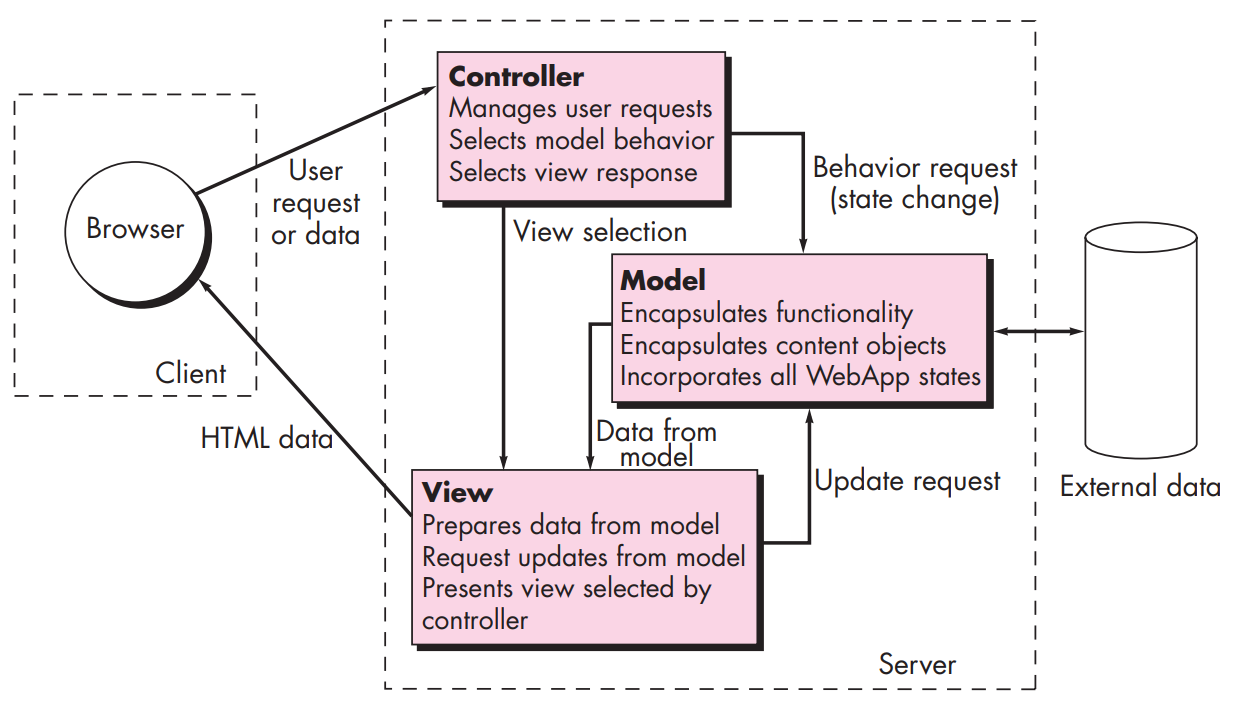
\includegraphics[width=0.68\textwidth]{arquitetura-mvc.png}
        \end{center}
    \label{dataMVCArchitecture}
    \legend{Fonte: \cite{pressman}}
\end{figure}

A arquitetura foi desenvolvida através, novamente, da linguagem de programação PHP. Para auxiliar na abstração e no desacoplamento entre os três módulos da arquitetura MVC, foi utilizado o motor de template Twig\footnote{\url{https://twig.symfony.com/} Acesso em outubro de 2018}. A ferramenta Twig  permite escrever um código mais conciso, com \textit{templates} mais legíveis e amigáveis para \textit{web designers} e, em vários casos, mais poderosos que \textit{templates} padrões do PHP \cite{symfonyBook}.

\begin{figure}[ht]
    \caption{Exemplo de \textit{template} padrão em PHP.}
        \begin{center}
            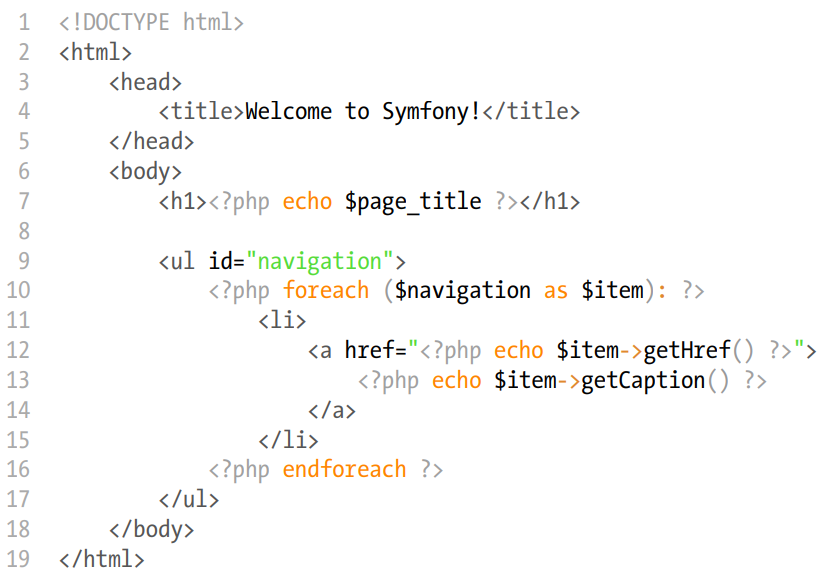
\includegraphics[width=0.68\textwidth]{twig-php.png}
        \end{center}
    \label{codeTemplatePHP}
    \legend{Fonte: \cite{symfonySensioLabs}}
\end{figure}

\bigskip

\begin{figure}[ht]
    \caption{Exemplo de \textit{template} em Twig .}
        \begin{center}
            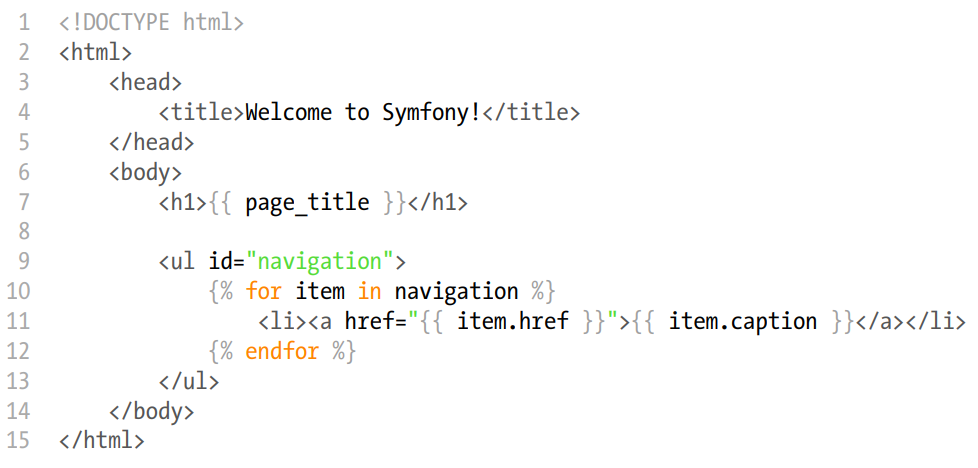
\includegraphics[width=0.68\textwidth]{figuras/twig-symf.png}
        \end{center}
    \label{codeTemplateTwig}
    \legend{Fonte: \cite{symfonySensioLabs}}
\end{figure}


\section{Projeto de Banco de dados}
\label{metodologiaBD}

O banco de dados utilizado na rede social foi o SGBD relacional MySQL. A ferramenta é livre, popular, robusta e amplamente utilizada em aplicações na Internet \footnote{\url{https://db-engines.com/en/ranking} Acesso em outubro de 2018}. O MySQL utiliza a linguagem SQL, \textit{Structured Query Language}, padrão dos bancos de dados relacionais para realizar consultas e atualizar informações nos dados armazenados pelo sistema \cite{sqlCompleteBook}.

O projeto de um banco de dados dá-se em duas fases: a modelagem conceitual, onde é construído um diagrama de entidade-relacionamento \cite{peterChen1976} e são capturadas as necessidades da organização independente de implementação; e o projeto lógico, que objetiva transformar o modelo conceitual em um modelo lógico, isto é, o modo como o banco de dados será implementado em um SGBD específico \cite{heuser}.

\subsection{Modelagem conceitual}
\label{BDModelagem}

A modelagem conceitual é utilizada para obter uma descrição abstrata, independente de implementação em computador, dos dados que serão armazenados no banco de dados. A técnica de modelagem de dados mais difundida e utilizada é a abordagem entidade-relacionamento (ER). \cite{heuser} Através dela, os modelos de dados são representados graficamente por um diagrama entidade-relacionamento (DER). A figura \ref{modelagemBDExemplol} apresenta um DER parcial presente na modelagem conceitual do sistema implementado.

\begin{figure}[h]
    \caption{Exemplo de modelagem conceitual.}
        \begin{center}
            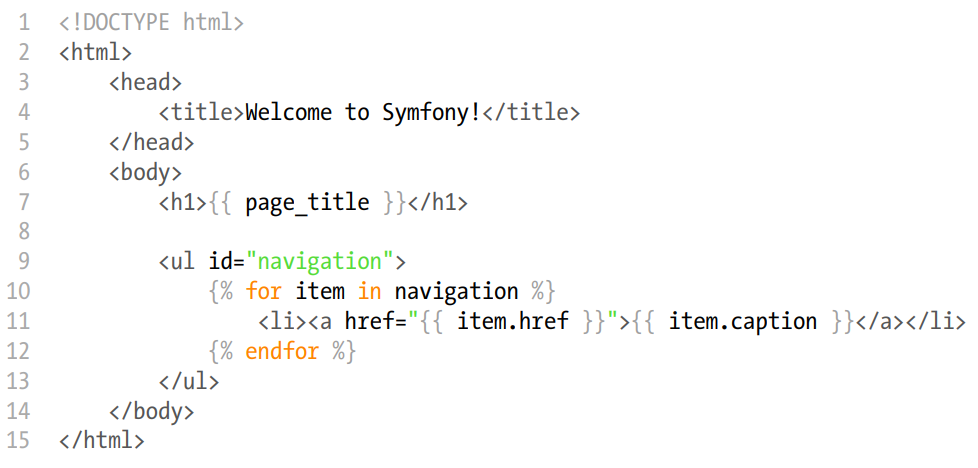
\includegraphics[width=0.68\textwidth]{figuras/twig-symf.png}
        \end{center}
    \label{modelagemBDExemplol}
    %\legend{Fonte: Autor}%
\end{figure}

\subsection{Projeto lógico}
\label{BDProjeto}

O projeto lógico consiste na transformação de um modelo ER em um modelo lógico. Este implementa de forma concreta, a nível de SGBD relacional, os dados representados no modelo ER.

Um determinado modelo ER pode ser implementado através de diversos modelos relacionais, que contém as informações especificadas pelo diagrama ER. Todos podem ser considerados uma implementação correta do modelo ER considerado. Entretanto, diferentes modelos relacionais podem resultar em diferentes performances do sistema construído sobre o banco de dados. 

No processo de transformação do modelo ER para o modelo relacional, foram utilizadas as seguintes regras de transformação \cite{heuser} a fim de obter uma melhor performance do sistema: 

\begin{itemize}
    \item Obter um banco de dados que permita boa performance de instruções de consulta e alteração do banco de dados.
    
    \item Obter um banco de dados que simplifique o desenvolvimento e a manutenção de aplicações.
    
    \item Evitar junções.
    
    \item Diminuir o número de chaves primárias.
    
    \item Evitar campos opcionais.
    
\end{itemize}

Os dois primeiros itens são alcançados naturalmente com as funcionalidades nativas do SGBD MySQL \cite{sqlCompleteBook}. As junções só ocorrem quando há uma relação 1:N entre duas entidades diferentes no sistema, minizando a quantidade de uso e consequente impacto dessas operações. Por fim, os dois últimos itens são respeitados com uma padronização de tabelas feitas para o projeto: todas possuem chave primária única e nenhum campo opcional. A figura \ref{modelagemBDLogicoExemplol} apresenta a transformação do modelo ER para o modelo relacional do exemplo apresentado na figura \ref{modelagemBDExemplol}.

\begin{figure}[h]
    \caption{Exemplo de modelagem relacional.}
        \begin{center}
            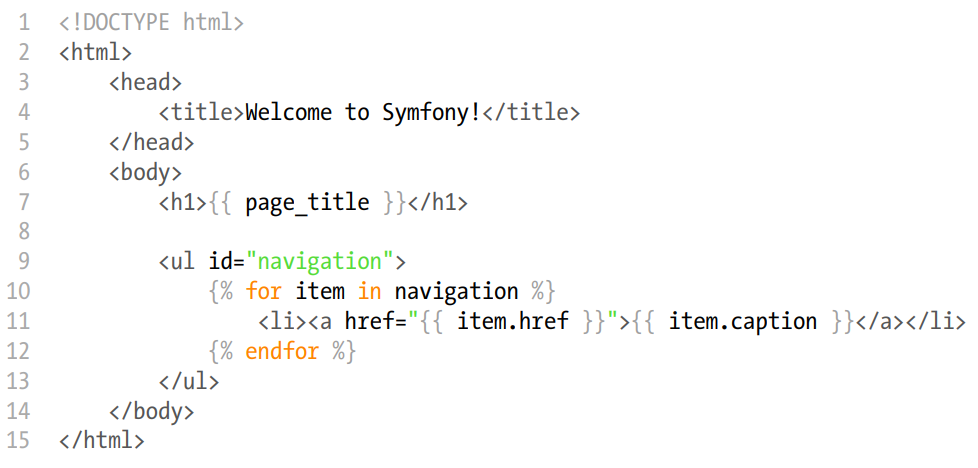
\includegraphics[width=0.68\textwidth]{figuras/twig-symf.png}
        \end{center}
    \label{modelagemBDLogicoExemplol}
    %\legend{Fonte: Autor}%
\end{figure}

\subsection{Criação do banco de dados}
\label{BDCriacao}

A etapa final do projeto de banco de dados consiste na implementação do modelo lógico de acordo com as regras e definições do SGBD escolhido. Para a transcrição do modelo em tabelas MySQL, foi utilizado o módulo do phpmyadmin que faz parte dos softwares e recursos instalados junto à pilha XAMPP (ver seção \ref{implementacaoConfig}). Através dessa ferramenta, é possível realizar consultas e  operações no SGBD como criação, edição e remoção de tabelas e registros.

\begin{figure}[h]
    \begin{adjustwidth}{-1in}{-.8in}
        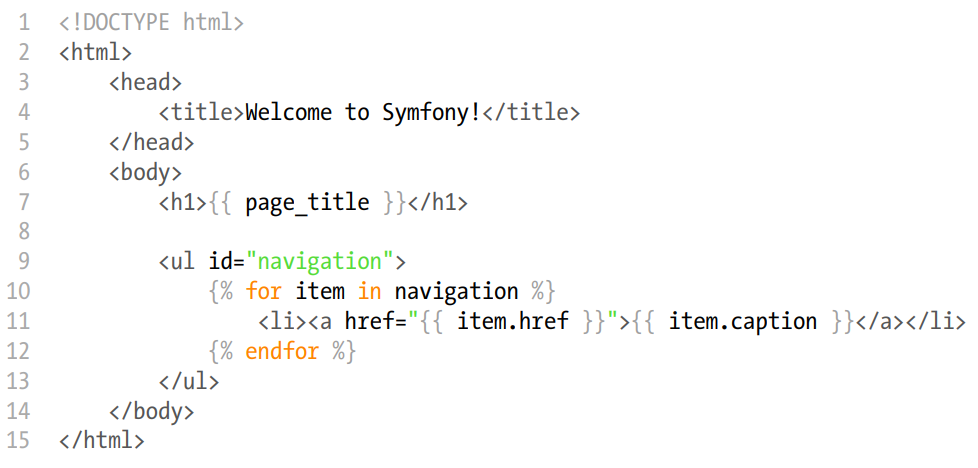
\includegraphics[width=0.68\textwidth]{figuras/twig-symf.png}
        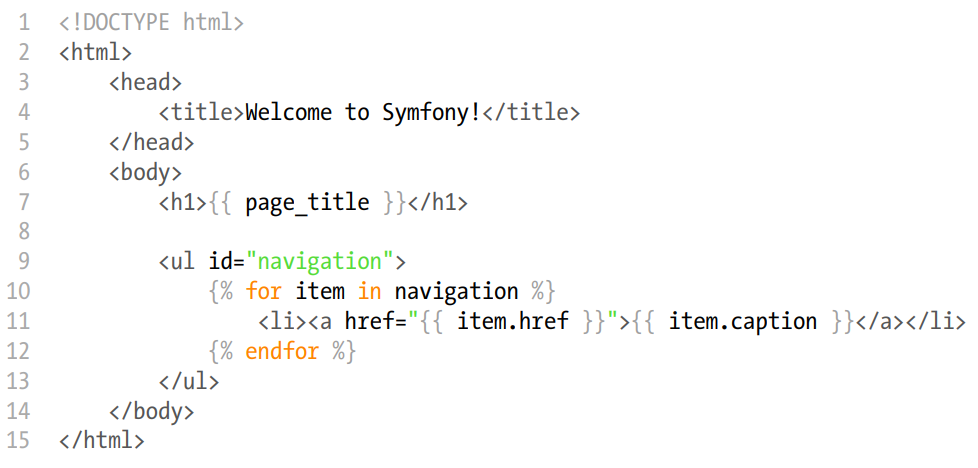
\includegraphics[width=0.68\textwidth]{figuras/twig-symf.png}
        \caption{Telas para criação do banco de dados e configuração da tabela [nome tabela].}
        \label{projetoImagens}
    \end{adjustwidth}
\end{figure}

Ao final deste processo, a implementação do banco de dados da rede social foi concluído com 17 tabelas, sendo elas:

\begin{itemize}
    \item \textbf{block:} registra uma ação de bloqueio entre dois usuários, representado pelo campo "id\_blocker", correspondente ao usuário bloqueante, e "id\_blocked", usuário bloqueado. São armazenadas ainda a informação de quando ocorreu a ação pelo campo "datetime\_created"\ e se o bloqueio está ativo ainda, visto que é uma ação reversível, através do campo "active".
    
    \item \textbf{comment:} tabela que gerencie os comentários em postagens de usuários. Composta pelos campos "id\_author", que é o \textit{id} do usuário que fez o comentário; "id\_post", \textit{id} da postagem onde foi feito o comentário; "text", o conteúdo propriamente do comentário; "datetime\_published"\ e "datetime\_last\_edit"\ correspondem às datas de postagem e última edição respectivamente; "active", indica se o comentário está visível ou não (excluído).
    
    \item \textbf{favorite:} 
    
    \item \textbf{follow:} registra uma ação de seguir entre dois usuários, representado pelo campo "id\_follower", correspondente ao usuário seguidor, e "id\_following", usuário seguido. São armazenadas ainda a informação de quando ocorreu a ação pelo campo "datetime\_created"\ e se o ato de seguir está ativo ainda, visto que é uma ação reversível, através do campo "active".
    
    \item \textbf{job:} representa uma vaga divulgada no sistema. "id\_author"\ guarda o \textit{id} do usuário que criou a vaga; "title"\ é o título da vaga; "category\_list"\ é uma lista de \textit{id} de categorias da tabela \textit{job\_category} que determinam as áreas de atuação da vaga; "resume"\ é uma descrição breve da vaga ofertada e "text", o texto completo; "skills"\ é a lista de habilidades que são interessantes o candidato possuir; "type"\ é o tipo de vaga ofertada: pode ser 0 para Monitoria, 1 para Bolsa administrativa, 2 para Bolsa de iniciação científica, 3 para Estágio, 4 para Trainee, 5 para Efetivo ou 6 para Voluntário; "modality"\ é a modalidade da vaga: 0 corresponde a uma vaga Presencial, 1 À distancia; "salary"\ representa a remuneração mensal; "semester"\ indica a partir de qual semestre o candidato estaria apto para se candidatar; "shift"\ registra em qual(is)  turno(s) o candidato terá de trabalhar, "is\_prae"\ é um campo booleano e representa se a vaga, caso seja uma bolsa da UFRGS, é exclusiva para beneficiários PRAE ou não; os campos "date\_start"\ e "date\_finish"\ indicam o período de vigência da vaga; "workload"\ corresponde ao total de horas semanais a vaga exige do candidato; os campos "location", "location\_city"\ e "location\_state" determinam o endereço da vaga; "need\_curriculum" especifica se a vaga exige \textit{curriculum vitae} do candidato; "need\_historic", de maneira semelhante, especifica se a vaga exige histórico escolhar do candidato; "datetime\_publication"\ e "datetime\_last\_edit"\ sinalizam as datas e horários que a vaga foi publicada e editada pela última vez respectivamente; por fim, o campo "active"\ guarda a informação se a vaga está disponível ou foi excluída.
    
    \item \textbf{job\_apply:} armazena informações quando um usuário manifesta interesse por uma vaga. O campo "id\_user" guarda o \textit{id} do usuário que realizou a ação e "id\_job", o \textit{id} da vaga em si. Adicionalmente, o campo "datetime\_created"\ registra a data e horário da ação e a coluna "active"\ indica se a manifestação de interesse está ativa ainda, pois o usuário pode desfazer sua ação.
    
    \item \textbf{job\_category:} essa tabela corresponde às áreas de atuação relacionadas a uma vaga. O campo "id" é utilizado como chave estrangeira para a lista presente em "category\_list" da tabela \textit{job}. 
    
    \item \textbf{log:}
    
    \item \textbf{post:} armazena todas as informações de um post feito por um usuário. O campo "id\_author" indica o \textit{id} do usuário que fez a postagem; "text" é o conteúdo da postagem; "datetime\_published"\ e "datetime\_last\_edit" representam as datas de criação e última edição da postagem respectivamente; "privacy"\ restringe a exibição do \textit{post}: 1, somente o autor pode olhar ou 0, todos os usuários; "allow\_comments"\ caso possua o valor 1, qualquer usuário pode comentar na postagem, caso contrário, nenhum pode; "active" é um indicativo se o post está visível ou não (foi excluído pelo autor).
    
    \item \textbf{post\_like:} registra a curtida de um usuário em um post. Os campos criados para a tabela são: "id\_user", referente ao \textit{id} do usuário; "id\_post", que diz respeito ao \textit{id} do post; "datetime\_created"\ informa a data e horário que ocorreu a ação do usuário; "active"\ sinaliza se a curtida está ativa, uma vez que a ação pode ser desfeita.
    
    \item \textbf{recommendation\_job:}
    \item \textbf{recommendation\_user:}
    
    \item \textbf{user:} tabela que salva todos os dados do usuário no sistema. É composta por x campos, sendo eles: "name"\ representa o nome do usuário no sistema; "age"\ é a idade do usuário; "born\_in\_city"\ e "born\_in\_state"\ indicam a cidade e o estado do local de nascimento respectivamente; "live\_in\_city"\ e "live\_in\_state"\ indicam a cidade e o estado onde o usuário reside no momento. "role"\ é a função deste no sistema sendo o valor 1 para Administrador; 2, professor; 3, técnico; 4, aluno. "phone"\ é o seu telefone de contato principal; "birthday"\ sua data de nascimento; "gender", seu sexo onde 0 é Masculino e 1, Feminino; "personal\_link" é um campo para o usuário divulgar sua página pessoal através de um link na Internet; "avatar"\ guarda o caminho relativo da imagem utilizada como foto de perfil do usuário no sistema; "email\_notification"\ sinaliza a preferência do usuário para receber e-mails de notificação do sistema; "show\_schollar\_info"\ e "show\_curriculum"\ são campos que, caso o usuário deseje, ele pode exibir as informações de histórico escolar e currículo no seu perfil respectivamente (valor 1 na coluna) ou omiti-los (valor 0); os campos "follower\_privacy"\ e "following\_privacy"\ restringem o acesso a informações sobre quem o usuário segue e quem o segue para usuários que não o seguem; "post\_privacy"\ é uma comodidade do sistema: indica a opção padrão durante criação de postagens; "datetime\_joined"\ salva a data de ingresso da primeira vez que o usuário fez \textit{login} no sistema. Este último e ainda os campos "id", "login", "email", "password" tiveram de ser simulados devido a restrições de integração do sistema (Ver seção \ref{redeLimitacao}).
    
    \item \textbf{user\_education:} relaciona um qualificação de ensino a um usuário. O campo "id\_user"\ é a chave estrangeira para o \textit{id} de um usuário na tabela \textit{user}. As colunas "title"\ e "subtitle"\ se referem ao grau de instrução ou informação de curso e a escola, universidade ou outra instituição de ensino onde o usuário estudou. "date\_start"\ e "date\_finish"\ guardam as informações do período que o usuário estudou na instituição. "location\_city"\ e "location\_state"\ mostram a cidade e o estado do ensino. O campo "selected"\ sinaliza se o trabalho é destaque; cada usuário pode destacar apenas um trabalho para ser exibida em informações simplificadas de perfil. Ainda, "active"\ informa se o dado está ativo ou foi excluído.
    
    \item \textbf{user\_job:} relaciona uma experiência de trabalho a um usuário. O campo "id\_user"\ é a chave estrangeira para o \textit{id} de um usuário na tabela \textit{user}. As colunas "title"\ e "company"\ se referem ao cargo e empresa onde o  usuário trabalhou. "date\_start"\ e "date\_finish"\ guardam as informações do período que o usuário trabalhou na empresa. "location\_city"\ e "location\_state"\ mostram a cidade e o estado do trabalho. A coluna "selected"\ sinaliza se o trabalho é destaque; cada usuário pode destacar apenas um trabalho para ser exibida em informações simplificadas de perfil. Por fim, "active"\ informa se o registro está ativo ou foi excluído.
    
    o idioma em questão. "level" indica o nível que o usuário possui, sendo 1 para Básico; 2, Intermediário; 3, Avançado; 4, Fluente; 5, Nativo. A coluna "active" informa se o dado está ativo ou foi excluído pelo usuário.
    
    \item \textbf{user\_language:} representa o conhecimento de um usuário sobre uma língua. O campo "title"\ é o idioma em questão. "level" indica o nível que o usuário possui, sendo 1 para Básico; 2, Intermediário; 3, Avançado; 4, Fluente; 5, Nativo. A coluna "active" informa se o dado está ativo ou foi excluído pelo usuário.
    
    \item \textbf{user\_skill:} representa o conhecimento de um usuário sobre uma língua. O campo "title"\ é o idioma em questão. "level" indica o nível que o usuário possui, sendo 1 para Iniciante; 2, Amador; 3, Júnior; 4, Pleno; 5, Sênior. "time" indica o tempo em anos que o usuário possui com essa habilidade. A coluna "active" informa se o dado está ativo ou foi excluído pelo usuário.
    
\end{itemize}

\section{Implementação}
\label{metodologiaImplementação}

A ferramenta foi implementada utilizando os conceitos de metodologia ágil de desenvolvimento, em especial, o SCRUM. O desenvolvimento da aplicação foi dividido em cinco fases: construção do \textit{framework} e  as entregas Inicial, Alfa, Beta e Final. Para uma maior organização durante toda a realização deste projeto, foi criado um repositório no GitHub\footnote{\url{https://github.com/jaflesch/tcc-ufrgs} Acesso em novembro de 2018} e definidas várias \textit{issues}, que agrupadas em \textit{milestones}, representavam um \textit{sprint}, uma etapa de desenvolvimento específico.

\subsection{Configuração do ambiente do trabalho}
\label{implementacaoConfig}

A construção do \textit{framework} focava em implementar conceitos abstratos da linguagem, arquitetura do sistema e funcionalidades básicas que seriam reaproveitadas nas etapas seguintes, como roteamento das páginas, configuração da conexão ao banco de dados e métodos genéricos.


\subsection{SCRUM}
\label{implementacaoSCRUM}

\subsection{Versão Inicial}
\label{implementacaoIR}

A entrega inicial priorizou a elaboração das principais telas do sistema, como a página Home, Feed de usuários, Vaga, Pesquisa e Login. A funcionalidade de realizar autenticação no sistema também foi implementada nesta etapa junto com consultas ao banco de dados que exibiam informações parciais de entidades como usuário e vaga.

\subsection{Versão Alfa}
\label{implementacaoAR}

A segunda etapa destinou-se à interação entre os usuários. Ao terminar da entrega alfa, já era possível seguir ou deixar de seguir um usuário, bloquear ou desbloquear um usuário, curtir ou descurtir um post e suas curtidas eram contabilizados dinamicamente, favoritar ou desfavoritar vaga, recomendar um usuário ou vaga. 

Sobre os aspectos visuais, foram desenvolvidas as páginas restantes: Configurações Gerais, Configurações de Privacidade, Usuários bloqueados, Seguidores; a barra de menu lateral ficou funcional e com animações ao abrir e fechar. Melhorias na experiência de usuário foram aplicadas com o aumento da área de clique em botões e no uso de cores mais contrastantes.

\subsection{Versão Beta}
\label{implementacaoBR}

A entrega Beta trouxe diversas melhorias às funcionalidades desenvolvidas. A pesquisa de vagas e de usuários ganharam novos filtros de modo a tornar a sua utilização mais inteligente, dinâmica e eficiente. Além disso, a interação quando um usuário manifestava interesse por vaga e a posterior gerência por parte de quem a divulgou foi finalizada. Por fim, a biblioteca de envio de e-mails para registrar e notificar ações importantes realizadas por usuários no sistema foi implementada.

No \textit{frontend}, iniciaram-se os primeiros passos para tratar as questões de responsividade em aparelhos móveis.

\subsection{Versão Final}
\label{implementacaoFR}

documentação e visual
aperfeiçoamento e otimização de funcionalidades


% ========== CAP 5 ==============
\chapter{A rede social Portal de Vagas}
\label{redeSocialPortal}

Este capitulo descreve as funcionalidades presentes e ausentes no prótotipo de rede social Portal de Vagas. Primeiramente, são é apresentado o funcionamento e todas interações possíveis em cada página do sistema. Em seguida, são listadas as limitações que a versão final do protótipo possui e, posteriormente, sugeridas melhorias como guia para trabalhos futuros. Por fim, é apresentado uma tabela comparativa, de maneira similar à seção [TRAB RELACIONADOS > COMPARAÇÃO]; porém, com o acréscimo do Portal de Vagas ao compartivo.

\section{Funcionamento}
\label{PDVFuncionamento}

Nesta seção será apresentado o funcionamento da rede social Portal de Vagas, explicando as funcionalidades e possibilidades de interação entre os usuários e as vagas ofertadas em todas as páginas do sistema, como a tela de login, as páginas inicial, de perfil de usuário, de vagas disponíveis e favoritas, de vaga específica, de configurações da conta de usuário, além da realização de consultas comuns e avançadas sobre vagas e usuários e do sistema de inscrição em vagas.

\subsection{Página de \textit{Login}}
\label{PDVFunLogin}

A rede social só pode ser utilizada através da autenticação de usuários cadastros no sistema. Dessa forma, caso algum usuário não autenticado tente acessar uma página interna e válida do sistema escrevendo diretamente sua URL no navegador, ele será redirecionando para a tela de \textit{login} automaticamente. Em contrapartida, caso o usuario já esteja autenticado e tente acessar a página de \textit{login} é redirecionado então para a página \textit{Home}.

A página apresenta um visual simples e objetivo, com o logotipo do INF e abaixo um formulário contendo um campo de nome de usuário ou e-mail e um para a senha. Contudo, como é mencionado na seção \ref{redeLimitacao}, por ser tratar de um protótipo, todos os usuários foram criados em um banco de dados exclusivo da aplicação. Dessa forma, não há de fato uma integração com o banco de dados de usuários da UFRGS, ou seja, não existe possibilidade, nesta implementação, de um usuário se autenticar com as mesmas credenciais em ambos os sistemas sem a criação prévia deste registro no banco do protótipo apresentado. 

Ainda, no final do formulário, existe um link para o usuário recuperar sua senha em caso de esquecimento. Como essa funcionalidade não seria necessária no protótipo, o link apenas redireciona o usuário para a página de recuperação de senha\footnote{\url{https://www.inf.ufrgs.br/portal/login.php\#resetpasswd} Acesso em novembro de 2018} na área de Administração de Rede do site do INF.

A Figura \ref{telaLoginImg} apresenta a página de \textit{login} com os campos de usuário e senha disponíveis para preenchimento. Só após a correta autenticação, as demais páginas da rede social ficam acessíveis.

\begin{figure}[h]
    \caption{Tela de \textit{login} do Portal de Vagas.}
        \begin{center}
            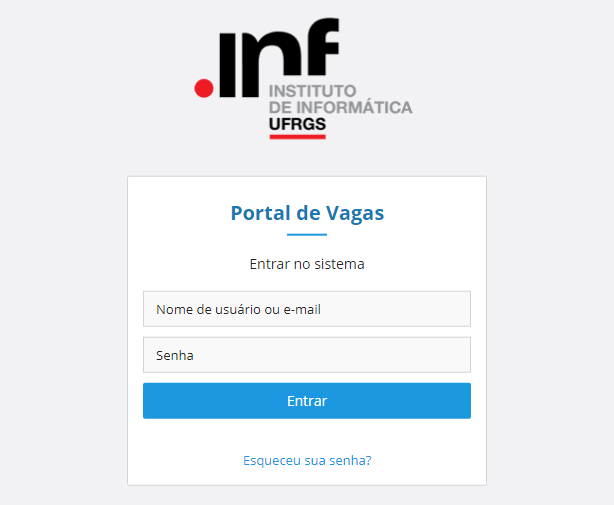
\includegraphics[width=0.85\textwidth]{figuras/tela_login.png}
        \end{center}
    \label{telaLoginImg}
    \legend{Fonte: Autor}
\end{figure}

\subsection{Página inicial}
\label{PDVFunFeed}

A página inicial do Portal de Vagas, acessada após o usuário se autenticar no sistema é composta por três seções: painel com dados resumidos do usuário, lista de postagens das pessoas seguidas na conta e painel de sugestões para seguir outros usuários e analisar vagas ofertadas, de forma a estimular o usuário a explorar a rede social. A Figura \ref{telaHome} exibe a Página inicial do sistema com suas três seções.

O painel com os dados resumidos apresenta a foto de perfil do usuário; seguido por seu nome; sua profissão, escolaridade ou local onde mora de acordo com os dados preenchidos; número de seguidores e desde quando realizou seu primeiro\textit{login} no sistema.

A lista de postagens começa com um campo de texto onde é possível o usuário realizar sua própria postagem que será exibida no \textit{feed} de seus seguidores. Da mesma forma, abaixo deste espaço, são apresentadas todas as postagens das pessoas que são seguidas pelo usuário. Nestas postagens, é possível curti-las e comentá-las também. Contudo, como a funcionalidade proposta seria uma alternativa aos e-mails de graduação, após comentar numa postagem, não é permitida a edição nem remoção deste, simulando assim um comportamento de serviço de \textit{webmail}.

Por fim, o painel de sugestões lista cinco usuários e vagas como sugestão para interação na rede social. Para as pessoas sugeridas, são ocultadas da lista as que o usuário já segue ou bloqueou. Além disso, ambas as listas são ordenadas pelo critério de relevância, isto é, as que possuem mais recomendações são apresentadas primeiro.

\begin{figure}[ht]
    \caption{Página inicial da rede social.}
        \begin{center}
            \includegraphics[width=1\textwidth]{figuras/arquitetura-centralizada-dados.png}
        \end{center}
    \label{telaHome}
    \legend{Fonte: Autor}
\end{figure}

\subsection{Página de perfil de usuário}
\label{PDVFunProfile}

A Página de perfil de usuário, semelhante a Página inicial, exibe informações sobre a pessoa que estamos acessando o perfil. Ela também é dividida em três seções principais, sendo elas: informações básicas de perfil, recomendações de outros usuários e um painel com sugestões de outras pessoas para interagir.

A seção de informações básicas pode ser editável contanto que o usuário autenticado esteja visitando o seu próprio perfil. Caso contrário, a página é apenas para leitura. Os dados são exibidos de forma completa e segmentados nos seguintes blocos: informações gerais, experiências profissionais, educação, habilidades profissionais e idiomas. Em informações gerais são apresentados um resumo dos dados mais importantes e recentes da pessoa como trabalho e educação mais recentes, localização, número de seguidores, desde quando está ativo no sistema e uma breve autodescrição. As experiências profissionais e educacionais são uma lista de dados ordenados da mais recente à mais antiga. Contudo, o usuário pode selecionar uma experiência para deixar destacada e ser a primeira a ser exibida (independente da ordenação inicial).Habilidades profissionais são uma lista de \textit{tags} acompanhadas do nível de experiência e tempo que possui tal conhecimento, apresentando uma lista bem sucinta das principais qualificações da pessoa. Por fim, de forma similar, há o bloco de idiomas que o usuário pode indicar e quantificar as línguas que ele possui fluência.

A seção de recomendações é um espaço para outras pessoas interagirem com o perfil do usuário visitado. Ali é possível recomendá-lo positivamente na rede social, qualificando-o individualmente e estimulando coletivamente as interações entre usuários. Além disso, é interessante considerar o cenário onde um professor esteja em dúvida sobre qual candidato aceitar em uma vaga ofertada: através das recomendações ele pode ter uma ideia mais concreta sobre a pessoa que estaria disposto a selecionar como seu bolsista, por exemplo. Ainda sobre a seção, um usuário só pode recomendar outros uma única vez e, obviamente, não pode recomendar a si mesmo.

Por último, o painel de pessoas sugeridas para o usuário seguir segue os mesmos critérios de ordenação da Página inicial. A diferença é que o número de sugestões é maior -dez pessoas- e não são sugeridas vagas na Página de perfil. A Figura \ref{telaUserProfile} apresenta a Página de perfil de usuário com todas as seções citadas.

\begin{figure}[ht]
    \caption{Página de perfil de usuário.}
        \begin{center}
            \includegraphics[width=1\textwidth]{figuras/arquitetura-centralizada-dados.png}
        \end{center}
    \label{telaUserProfile}
    \legend{Fonte: Autor}
\end{figure}

\subsection{Página de vagas disponíveis}
\label{PDVFunVagas}

A Página de vagas fornece ao usuário uma lista de todas as vagas disponíveis no sistema, sejam elas bolsa de monitoria, iniciação científica, estágio, ou até mesmo de efetivo. Uma das propostas do Portal de Vagas é uma releitura da página de vagas ofertadas no Mural de Bolsas.A estrutura da página é composta por duas seções principais: a área de filtros de pesquisa e a lista de vagas disponíveis.

A área de filtros foi expandida em relação ao Mural de Bolsas. Agora é possível filtrar por localidade e também incorporar as funcionalidades integradas de vagas que exigem currículos e/ou histórico escolar. Além disso, é possível selecionar o método de ordenação: mais relevantes, melhores avaliados, mais recentes e mais antigos. No MB a listagem era ordenada pelas vagas mais recentes primeiro. Por padrão, a lista de filtros é oculta e, se o usuário sentir necessidade, pode expandi-la e aplicar os filtros desejados. A Figura \ref{telaFiltros} exibe a seção em formato expandido com todos os campos possíveis.

\begin{figure}[ht]
    \caption{Lista de filtros expandidos.}
        \begin{center}
            \includegraphics[width=1\textwidth]{figuras/arquitetura-centralizada-dados.png}
        \end{center}
    \label{telaFiltros}
    \legend{Fonte: Autor}
\end{figure}

A lista de vagas é apresentada em uma visão de \textit{cards}, onde cada cartão apresenta as conjunto de informações compacto com "título", "localização", "áreas de atuação", "resumo", "remuneração" e "carga horária". Além disso, possui um botão para salvar a vaga na lista de favoritos do usuário; o botão "Candidatar-se" para se inscrever numa vaga disponível (ver seção \ref{PDVFunInscricoes}) e o botão "Ver mais" que abre a página da vaga selecionada com todas suas informações e recomendações. A Figura \ref{telaVagasLista} apresenta a visualização de vagas disponíveis.

\begin{figure}[ht]
    \caption{Lista de vagas disponíveis em formato de \textit{card}.}
        \begin{center}
            \includegraphics[width=1\textwidth]{figuras/arquitetura-centralizada-dados.png}
        \end{center}
    \label{telaVagasLista}
    \legend{Fonte: Autor}
\end{figure}

\subsection{Página de vaga específica}
\label{PDVFunVaga}

A Página de vaga específica é uma versão completa dos \textit{cards} apresentados na página de Lista de vagas. Essa página apresenta três seções: a área de informação de vaga, o painel com lista de vagas relacionadas e a área de recomendações. Se o usuário que acessa a página é o próprio autor da vaga, existe ainda uma quarta seção: a de candidatos inscritos. A Figura \ref{telaVagaCompleta} exibe a página da Vaga de maneira completa com todas as seções disponíveis.

A área de informação da vaga, em ordem de exibição, contempla os seguintes dados: "título da vaga", "localização", "áreas de interesse", "autor da vaga", "descrição completa", "modalidade", "tipo de vaga", "experiência exigida", "carga horária", "turnos", "data de início", "duração", "exigência de currículo", "exigência de histórico escolar", "benefício PRAE". Alguns dados podem ser omitidos caso o autor da vaga opte por deixar alguma informação opcional em branco. Ao final, existe um botão de "Candidatar-se" também caso o usuário não tenha se inscrito na vaga ainda.

A seção de recomendações é uma lista com todas as recomendações enviadas por usuários que decidiram avaliar positivamente a vaga ofertada. Cada recomendação contém dados básicos do autor e o texto explicando o motivo da avaliação. Os usuários podem recomendar cada vaga uma única vez.

No canto superior direito, existe também um painel com uma lista de vagas semelhantes que possam interessar o usuário, facilitando assim o fluxo de navegação. O critério de ordenação é a relevância da vaga, isto é, as que possuem mais recomendações e mais favoritadas, vêm primeiro.

Por fim, para a situação em que o usuário autenticado é também o autor da vaga...

\begin{figure}[ht]
    \caption{Página de vaga com todas informações disponíveis.}
        \begin{center}
            \includegraphics[width=1\textwidth]{figuras/arquitetura-centralizada-dados.png}
        \end{center}
    \label{telaVagaCompleta}
    \legend{Fonte: Autor}
\end{figure}

\subsection{Página de Favoritos}
\label{PDVFunFavoritos}

A Página de favoritos é apenas uma comodidade oferecida pelo sistema. Nela se encontram todas as vagas que estão favoritadas pelo usuário. Dessa forma, a página já oferece uma lista de vagas que atendem a esse critério inicial. Além disso, os filtros tradicionais presentes na página de Vagas também estão disponíveis para uso e posterior refinamento de pesquisa. A Figura \ref{telaVagaFav} apresenta todas as vagas favoritas pelo usuário: repare que o ícone de estrela fica destacado na cor azul.

\begin{figure}[ht]
    \caption{Página de vagas favoritas do usuário.}
        \begin{center}
            \includegraphics[width=1\textwidth]{figuras/arquitetura-centralizada-dados.png}
        \end{center}
    \label{telaVagaFav}
    \legend{Fonte: Autor}
\end{figure}

\subsection{Página de inscrições}
\label{PDVFunInscricoes}

A Página de inscrições apresenta a lista de inscrições dos usuários em vagas ofertadas pelo sistema. Ela apresenta três seções importantes: a área de filtro, a lista de inscrições e o painel de sugestões. duas exibições diferentes que levam em conta o papel do usuário no sistema. Se ele for um aluno, a página apresentará uma lista com todas as vagas que este se inscreveu. Se for professor, então a lista será de todos os alunos que se inscreveram nas vagas criadas por ele.

Em ambos os papéis, a área de filtros apresenta o mesmo comportamento: ela fornece um formulário com 3 \textit{checkboxes} que descrevem a situação em que se encontra a instrição. São elas: "em avaliação" (ou "avaliação pendente" se for professor), "aprovado" e "reprovado". Por padrão, a opção que vem marcada filtra os resultados para exibir apenas as inscrições em andamento, pois é a informação de maior interesse dos autores e candidatos da vaga.

O painel de sugestões mantém o mesmo princípio das páginas anteriores e exibe uma lista com as vagas ofertadas na rede social ordenadas da maior para a menor relevância.

A principal diferença das seções ocorre na listagem. Quando um aluno se candidata a uma vaga, o professor recebe um e-mail notificando-o sobre uma nova inscrição. Nesse momento, o \textit{status} da inscrição é marcado como "em avaliação". Quando o professor avalia a inscrição e opta por aprovar ou reprovar a candidatura, o aluno também é notificado por e-mail. As diferenças entre as telas para os dois usuários estão representadas nas Figuras \ref{telaInscrAluno} e \ref{telaInscrProf}.

\begin{figure}[h]
    \caption{Tela de inscrições para alunos.}
        \begin{center}
            \includegraphics[width=0.75\textwidth]{figuras/arquitetura-centralizada-dados.png}
        \end{center}
    \label{telaInscrAluno}
    \legend{Fonte: Autor}
\end{figure}

\begin{figure}[h]
    \caption{Tela de inscrições para professores.}
        \begin{center}
            \includegraphics[width=0.75\textwidth]{figuras/arquitetura-centralizada-dados.png}
        \end{center}
    \label{telaInscrProf}
    \legend{Fonte: Autor}
\end{figure}

\subsection{Página de pesquisa}
\label{PDVFunPesquisa}

Sempre que o usuário sentir necessidade de procurar por usuários ou vagas de um modo mais genérico, ele pode realizar a consulta digitando um termo de interesse no campo de pesquisa no cabeçalho de todas as páginas. Assim, ele será direcionado para a página de Pesquisa que exibe todos resultados encontrados tanto nas vagas quanto em usuários cadastrados no sistema. A Figura \ref{PDVPesquisaTela} mostra a tela de resultados encontrados na págia de Pesquisa.

A página ainda fornece ao usuário a possibilidade filtrar os resultados por "pessoas" ou "vagas". Além disso, no canto direito, existe um painel listando os 10 termos mais recentes e pesquisados na rede social, ordenados do maior para o menor.

\begin{figure}[ht]
    \caption{Página de Pesquisa: exemplo de tela com os resultados para a pesquisa pelo termo "lsa". }
        \begin{center}
            \includegraphics[width=0.68\textwidth]{arquitetura-centralizada-dados.png}
        \end{center}
    \label{PDVPesquisaTela}
    \legend{Fonte: Autor}
\end{figure}

\subsection{Páginas de preferências do usuário}
\label{PDVFunConfiguracoes}

As páginas de preferências são um agregado de opções que a rede social oferece de forma que os usuários possam escolher o comportamento do Portal de Vagas em determinadas ações como: exibição ou não de currículo e histórico escolar, nome de exibição no sistema, \textit{e-mail} para notificações do sistema.

Por padrão, a primeira tela é sempre a de Configurações gerais. Ao lado esquerdo, existe um painel com uma lista para acesso rápido de todas as opções oferecidas ao usuário. Ao lado direito, são exibidos campos do formulário da página em questão. Foi adicionado também um destaque no link de acesso rápido referente à página em questão. Isto é, o \textit{link} fica em negrito, sublinhado e azul.

\subsubsection{Configurações gerais}
\label{PDVFunConfiguracoesGeral}

A tela de Configurações gerais apresenta um formulário com quatro campos. O primeiro é o nome de exibição do usuário no sistema. O campo de \textit{e-mail} serve como complemento aos já fornecidos pelo INF e UFRGS. Neste caso, a ideia é o usuário ter a possibilidade de cadastrar um e-mail em uma plataforma que ele utilize com maior frequência, pois facilitaria o recebimento de notificações enviadas pelo Portal de Vagas. O telefone é um campo não obrigatório e só é exibido para o autor de uma vaga ofertada caso o usuário demonstre interesse por esta. Por fim, há o campo de idioma onde o usuário pode alternar entre as diferentes linguagens ofertadas pela rede social (para o protótipo apenas a lingua portuguesa está disponível). A Figura \ref{telaConfigGeral} apresenta a tela de Configurações gerais.

\begin{figure}[ht]
    \caption{Tela de Configurações gerais.}
        \begin{center}
            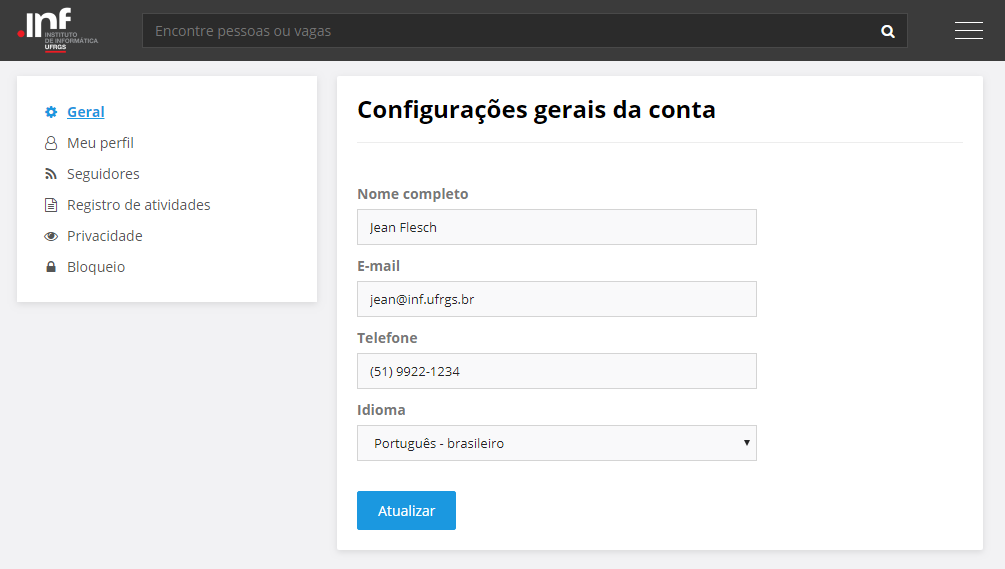
\includegraphics[width=1\textwidth]{figuras/config_01.png}
        \end{center}
    \label{telaConfigGeral}
    \legend{Fonte: Autor}
\end{figure}

\subsubsection{Lista de seguidores}
\label{PDVFunConfiguracoesListaSeguidores}

A página de Lista de seguidores exibe todos os seguidores do usuário, de maneira ordenada, do mais recente ao mais antigo. Existem duas seções na página: a primeira é um parágrafo informativo sobre como as configurações de privacidade afetam na exibição da lista de seguidores para outros usuários do sistema; a segunda é, de fato, a lista de usuários seguidores. Cada registro possui um link direto para o perfil do seguidor. A Figura \ref{telaConfigSeguidores} exibe a página da Lista de seguidores.

\begin{figure}[ht]
    \caption{Tela de seguidores do usuário.}
        \begin{center}
            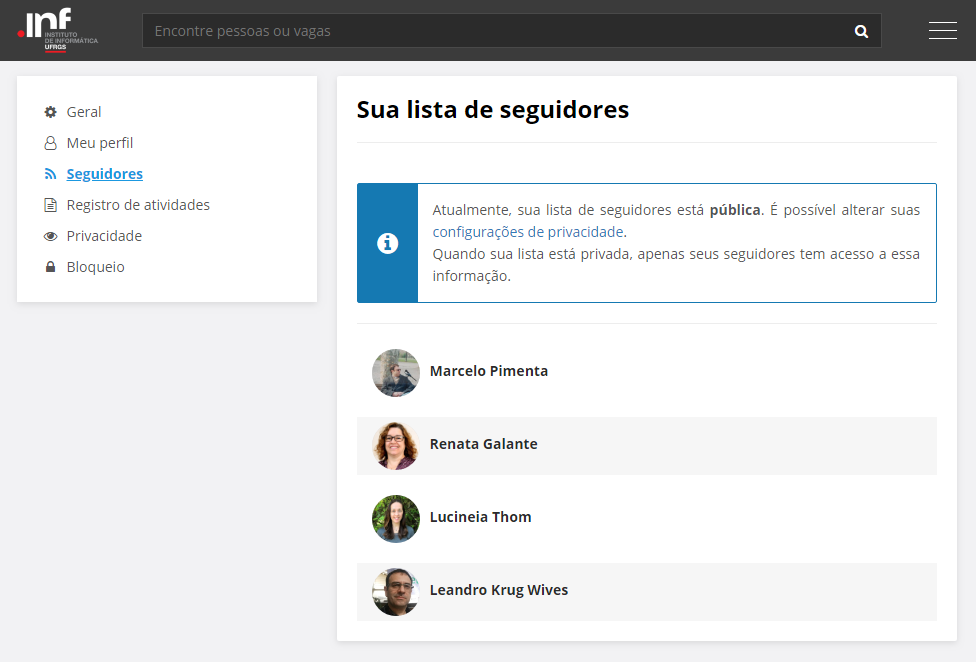
\includegraphics[width=1\textwidth]{figuras/config_05.png}
        \end{center}
    \label{telaConfigSeguidores}
    \legend{Fonte: Autor}
\end{figure}

\subsubsection{Registro de atividades}
\label{PDVFunConfiguracoesLog}

A página de Registro de atividades funciona como um histórico de todas as ações significativas de um usuário no Portal de Vagas. As ações são apresentadas em um formato de linha do tempo onde o mais recente é o primeiro a ser exibido. Cada registro possui texto e ícones personalizadas para diferenciação.

Os seguintes eventos são considerados ações significativas e, consequentemente, exibidos no Registro de atividades:

\begin{itemize}
    \item Realizar primeiro login no sistema;
    \item Atualizar foto de perfil;
    \item Curtir uma postagem;
    \item Comentar em uma postagem;
    \item Favoritar ou desfavoritar uma vaga;
    \item Demonstrar interesse numa vaga;
    \item Recomendar usuário ou vaga
    \item Seguir ou deixar de seguir usuário;
    \item Bloquear ou desbloquear usuário;
    \item Aprovar ou reprovar um candidato numa vaga;
    \item Criar, editar ou deletar vaga;
\end{itemize}

\begin{figure}[h]
    \caption{Tela de Registro de atividades do usuário.}
        \begin{center}
            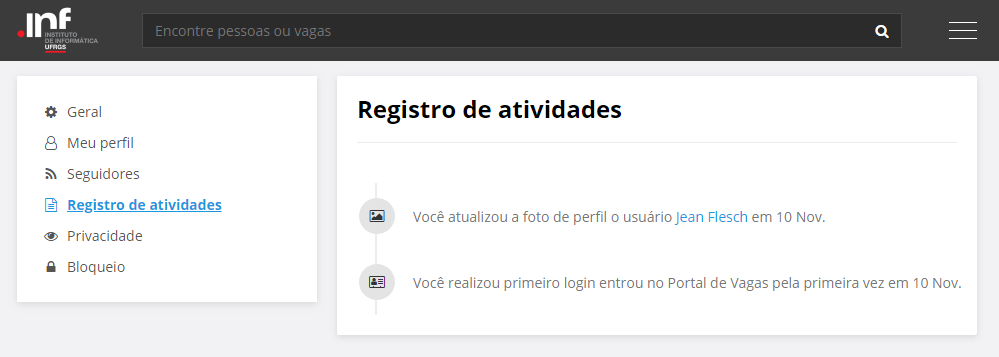
\includegraphics[width=1\textwidth]{figuras/config_03.png}
        \end{center}
    \label{telaConfigLog}
    \legend{Fonte: Autor}
\end{figure}

\subsubsection{Configurações de privacidade}
\label{PDVFunConfiguracoesPrivacidade}

A página de Configurações de privacidade fornece flexibilidade ao usuário para que ele possa controlar o quais informações são visíveis às demais pessoas da rede social. Para este protótipo, foram propostas as seguintes opções de privacidade:

\begin{itemize}
    \item \textbf{Visibilidade das publicações:} todos os usuários têm acesso (público) ou apenas seguidores (privado);
    
    \item \textbf{Histórico escolar:} se o usuário deixar visível, outras pessoas poderão ver os conceitos deste em sua página de perfil. Caso contrário, a informação é oculta. Independentemente da escolha do usuário nesta opção, quando ele se candidata a uma vaga que exige histórico escolar, seus dados são enviados ao autor da vaga.
    
    \item \textbf{Currículo:} o funcionamento é o mesmo que na opção de histórico escolar: o usuário pode ocultar ou não a informação em seu perfil, mas se ele se candidata a uma vaga que exige currículo, a informação é enviada automaticamente ao autor da vaga.
    
    \item \textbf{Visibilidade da lista de seguidores:} todos os usuários têm acesso (público) ou apenas seguidores (privado);
    
    \item \textbf{Visibilidade da lista de seguidos:} todos os usuários têm acesso (público) ou apenas seguidores (privado)
\end{itemize}

\begin{figure}[ht]
    \caption{Tela de Configurações de privacidade.}
        \begin{center}
            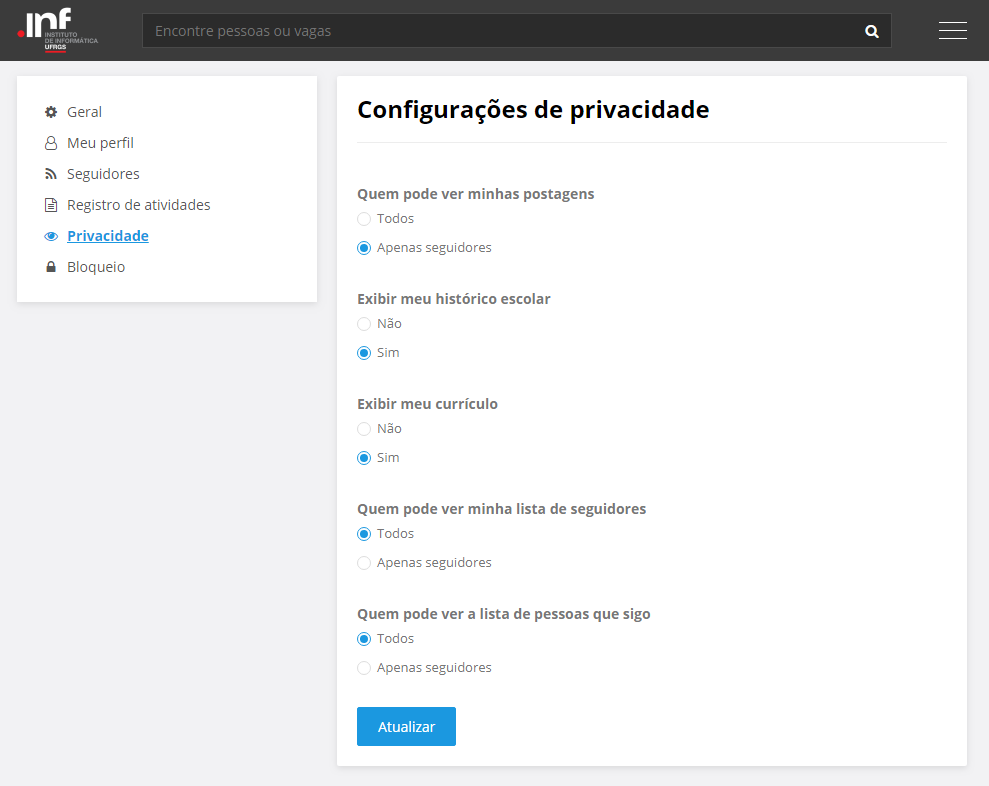
\includegraphics[width=0.68\textwidth]{figuras/config_02.png}
        \end{center}
    \label{telaConfigPrivacidade}
    \legend{Fonte: Autor}
\end{figure}

\subsubsection{Lista de bloqueados}
\label{PDVFunConfiguracoesBloq}

Assim como a Lista de seguidores, a página com a Lista de bloqueados é uma funcionalidade que prioriza uma melhor experiência de usuário. Nesta situação, a página apresenta também duas seções: a primeira informa ao usuário as consequências de adicionar outra pessoa na sua lista de bloqueados; a segunda, é a lista de todos os usuários bloqueados.

As principais consequências de bloquear um usuário são: ele não aparecerá na lista de sugestões de usuários para seguir; as publicações dele ficam ocultas, não é possível comentar em posts criados por ele nem recomendar vagas que ele publicar. Entretanto, o bloqueio não é bidirecional, isto é, ele ainda poderá ter acesso a quaisquer informações compartilhadas publicamente. A Figura \ref{telaConfigBloq} exibe o visual da página de usuários bloqueados.

\begin{figure}[ht]
    \caption{Tela de usuário bloqueados.}
        \begin{center}
            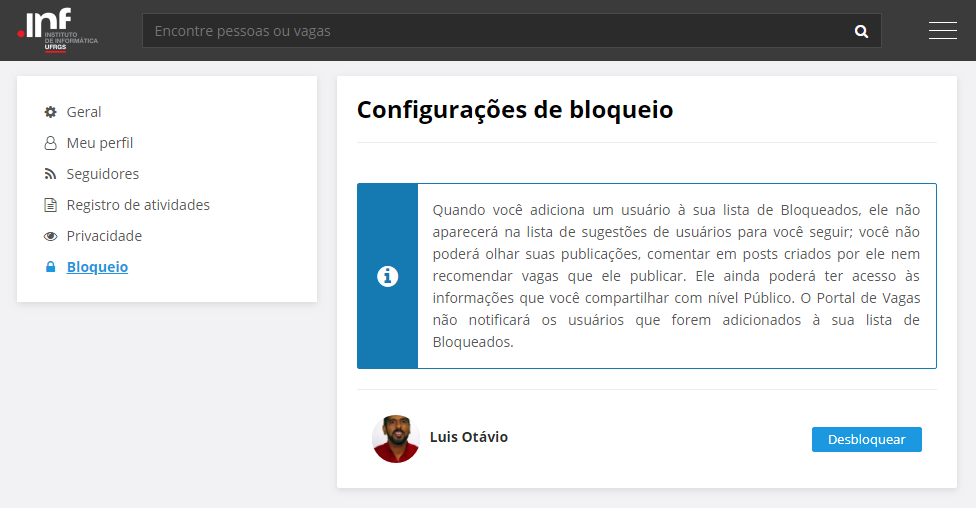
\includegraphics[width=0.95\textwidth]{figuras/config_04.png}
        \end{center}
    \label{telaConfigBloq}
    \legend{Fonte: Autor}
\end{figure}

\section{Limitações e trabalhos futuros}
\label{redeLimitacao}

A rede social Portal de Vagas, por se tratar de um protótipo, possui limitações de sistema. Para tornar possível sua aplicação completa, são necessários alguns passos adicionais. O primeiro e mais importante seria a realização de uma integração real com as demais ferramentas utilizadas pela UFRGS. Por exemplo: a funcionalidade de obter o histórico escolar do aluno e enviar seu currículo automaticamente por e-mail ao responsável pela vaga foi implementada no protótipo com o envio de um arquivo estático em formato \textit{.pdf}. Na versão final, um passo adicional seria realizar uma consulta ao banco de dados utilizado no Portal do Aluno e retornar os valores que lá são apresentados. Além disso, outras ferramentas como o próprio Moodle e o \textit{Webmail} poderiam ser utilizados para aumentar a experiência de usuário. 

O Moodle mantém as informações de turmas que o aluno cursou em sua jornada acadêmica. Dessa forma, o critério de ordenação por relevância em vagas poderia se valer de uma inteligência artificial mais sofisticada e atribuir um peso maior para vagas relacionadas às disciplinas cursadas. Essa estratégia seria bastante útil com cadeiras eletivas, visto que elas abordam assuntos específicos de áreas de conhecimento e ajudam a descrever o perfil do aluno mais precisamente. 

O \textit{Webmail} é um interface online que oferece serviço de leitura e envio de e-mails utilizando o navegador. No INF, alunos de graduação fazem parte do grupo \textit{graduacao@inf.ufrgs.br} e sempre que um e-mail é enviado ao grupo, todos seus participantes o recebem. Dessa forma, quando um professor divulga uma nova vaga ofertada, o sistema poderia automaticamente enviar e-mails para a lista da graduação. De maneira similar, quando um usuário faz uma postagem, ele pode escolher se deseja também notificar os usuários pelo e-mail da graduação, além dos seus seguidores na rede social.

Do ponto de vista do sistema como rede social, existe uma variedade de funcionalidades que podem ser estentidas e adicionadas, visando o aumento da experiência do usuário final. Compartilhar uma postagem ou uma vaga, curtir comentários e recomendações, aumentar o número de configurações da conta, podendo restringir o acesso a campos individuais do perfil de usuário são apenas alguns exemplos.

\section{Comparação}
\label{redeComparacao}

[]Utilizar a mesma tabela do capitulo de trabalhos relacionados, mas adicionando o PDV...]

% ========== CAP 6 ==============
\chapter{Avaliação com os usuários}
\label{Avaliação}

Este capítulo é dedicado a apresentar o experimento realizado com os usuários.  A avaliação consistiu na realização de uma sequência pré-definida de tarefas em duas plataformas diferentes: o prótotipo de rede social implementado neste trabalho, Portal de Vagas, e a ferramenta já existente utilizada na UFRGS: o Mural de Bolsas. Para a comparação entre os dois sistemas propostos, o experimento utilizou o \textit{A-B testing}. 

No final deste capítulo são exibidos os resultados obtidos com a avaliação e duas análises destes: uma objetiva e outra subjetiva.

\section{Ambiente dos experimentos}
\label{avaliacaoAmbiente}

Para a aplicação dos experimentos, os usuários utilizaram de equipamento apenas um computador com acesso à Internet. Dois ambientes foram escolhidos para os testes: aos usuários que realizaram o experimento na UFRGS, optou-se por utilizar as dependências dos laboratórios do Instituto de Informática; aos usuários externos à universidade, o experimento foi aplicado em uma sala isolada. Ambos os locais escolhidos contaram com ausência de interferência externa, isto é, barulhos indesejáveis que comprometessem a concentração do usuário, minimizando assim, o incômodo e eventual cansaço dos participantes.

\section{Perfil dos usuários}
\label{avaliacaoPefil}

Todos os participantes assinaram um termo de consentimento livre e preencheram um formulário (vide Apêndice \ref{appendFormPortal}) de caracterização antes do experimento. Participaram X voluntários ao todo (e todos completaram os testes / mas X desistiram por motivos de... e sua participação, por ser incompleta, foi descartada nas análises posteriores). Dos X participantes que completaram todos as etapas da avaliação, X eram homens e Y mulheres; com faixa etária de X a X anos; com escolaridade majoritariamente X, (X pessoas), seguido por Y e Z. Dos X candidatos com nível superior (completo, incompleto) ou com pós-graduação, X eram da área de, Y da, Z da .... . No que tange ao conhecimento dos usuários em tecnologias, a maioria apresenta experiência com Internet, redes sociais e a minoria possui experiência com a rede social LinkedIn.

As Figuras x a y apresentam características gerais dos voluntários que contribuíram para o experimento.

\section{Protocolo de testes}
\label{avaliacaoProtocolo}

Para cada usuário, são realizadas as seguintes etapas:

\begin{itemize}
    \item \textbf{Formulário pré-teste:} são feitas perguntas para caracterização do usuário como \textit{"idade"}, \textit{"sexo"}, \textit{"nível de escolaridade"}, \textit{"área de formação superior"}, \textit{"experiência com Internet"}, \textit{"experiência com redes sociais"} e \textit{"experiência com LinkedIn"};
    
    \item \textbf{Etapa 1:} o usuário é submetido a realização de uma sequência de atividades na plataforma. São elas:
        \begin{itemize}
            \item atividade 1
            \item atividade 2
            \item atividade N
        \end{itemize}
        
    \item \textbf{Formulário pós-etapa:} objetiva saber opiniões do experimento realizado, conforme descrito no Apêndice \ref{appendFormStepPortal};
    
    \item \textbf{Etapa 2:} novamente, o usuário é submetido a realização da mesma sequência de atividades anteriores. Porém, na outra plataforma. São elas:
        \begin{itemize}
            \item atividade 1
            \item atividade 2
            \item atividade N
        \end{itemize}
        
    \item \textbf{Formulário pós-etapa:} objetiva saber opiniões do experimento realizado, conforme descrito no Apêndice \ref{appendFormStepPortal};
    
    \item \textbf{Formulário pós-testes:} busca comparar as duas etapas completadas pelo usuário, conforme descrito no Apêndice \ref{appendFormFinalPortal}.
\end{itemize}

Para aplicar o teste da maneira mais neutra possível, seguindo o protocolo do \textit{A-B testing}, foi alternada a ordem das Etapas 1 e 2. Metade da população realizou as tarefas no Mural de Bolsas primeiro e depois no Portal de Vagas. A outra metade, o oposto.


\section{Análise geral dos resultados}
\label{avaliacaoAnalise}

Os resultados avaliados serão divididos em duas categorias: resultados subjetivos e resultados objetivos. O primeiro avalia as respostas e opinião dos participantes nos questionários. Já o segundo avalia o desempenho destes a partir da observação de \textit{logs} gerados durante a execução dos testes.


\subsection{Análise Subjetiva}
\label {avaliacaoAnaliseSubjetiva}

Analisando as respostas obtidas durante a primeira etapa do teste, sobre o questionário de caracterização dos usuários, podemos destacar (escolaridade, experiência com internet, redes sociais e linkedin…). Esse resultado já era esperado e o questionário foi feito com o intuito de englobar um nicho de participantes genérico, isto é, sem ter obrigatoriamente um grande conhecimento em tecnologias, visto que, aplicações como redes sociais possuem os mais variados perfis de usuário. Portanto, nenhum participante foi descartado a partir das respostas fornecidas nesta etapa, já que foram procuradas justamente pessoas com essas características.
Ao final de cada sequência de atividades propostas numa plataforma, foi aplicado um questionário para o participante informar o nível de dificuldade das tarefas. Como foi utilizado o protocolo \textit{AB-testing}, um grupo de usuários realizou o experimento primeiro com o Portal de Vagas e, posteriormente, o Mural de Bolsas. O outro grupo realizou o experimento na ordem inversa. 

Sendo assim, X consideram a dificuldade maior em Y. Entre as principais dificuldades relatadas foram X, Y, Z. A outra parcela dos usuários, embora em menor representatividade, alegaram que a dificuldade foi maior em X pelos seguintes motivos: …

Ainda, o questionário abordou a seguinte questão “De forma geral, como você avalia seu desempenho executando as atividades na plataforma?”. O objetivo é analisar o grau de satisfação do participante ao concluir todas as tarefas e identificar se existe alguma relação com a dificuldade mencionada anteriormente. Para essa questão, a maioria, X, respondeu que considera seu desempenho <...>.

A última etapa do questionário instigou os participantes a compararem as duas plataformas, uma vez que eles tinham uma opinião mais sólida após realizarem os dois testes. X respondeu que notou uma diferença de dificuldade entre as plataformas. Destes, Y considerou a plataforma X mais difícil que a Y.


\subsection{Análise Objetiva}
\label {avaliacaoAnaliseObjetiva}

Nos testes foram salvos \textit{logs} para armazenar a quantidade de tempo investida por cada participante nas atividades propostas nas duas plataformas. Dessa forma, cada \textit{log} é composto ao todo por X campos, sendo Y para cada plataforma.

Posteriormente, foi calculada a média e o desvio padrão dos tempos obtidos por cada atividade nas duas plataformas, como podemos observar na tabela \ref{tableAvalObj}.

\begin{table}[h]
    \begin{adjustwidth}{-0.7in}{-0.7in}
    \begin{center}
    \begin{tabular}{ccccccccccccc}
    \hline
     & Plataforma & Tempo médio & Desvio padrão \\
    \hline
    Atividade 1 & MB & 1s & 1 \\
    Atividade 1 & PDV & 1s & 1 \\
    Atividade n & MB & 1s & 1 \\
    Atividade n & PDV & 1s & 1 \\
    \hline
    \end{tabular}
    \end{center}
    \end{adjustwidth}
    \bigskip
    \legend{Tabela com os tempos obtidos pelos participantes em cada atividade nas duas plataformas.}
    \label{tableAvalObj}
\end{table}

Observamos que ... <análise dos tempos>

Portanto, podemos concluir que ... <conclusão sobre tempos>

% ============== CONCLUSÃO =========================
\chapter{Conclusões}
\label{conclusao}

Neste trabalho foi apresentado o Portal de Vagas, um protótipo de rede social desenvolvido para explorar novas alternativas para a divulgação de bolsas e estágios na universidade. Além disso, a plataforma também simulou a integração com outras ferramentas já utilizadas pela UFRGS, como o Moodle, o Portal do Aluno e o Webmail em um ambiente de dados centralizado.

O trabalho começou com um estudo de trabalhos relacionados, em especial o Mural de Bolsas, onde foram detectadas funcionalidades essenciais para a rede social, que serviram de base para a análise de requisitos. Posteriormente, foi definida a metodologia ágil para o desenvolvimento da aplicação, dividida em quatro sprints baseadas em critérios de prioridade. 

A primeira entrega priorizou a funcionalidade de login e a construção das páginas básicas da rede social. A segunda, focou nas interações entre usuários como curtir, postar, seguir e bloquear e filtros padrões na busca de vagas. A terceira, finalizou as demais interações de usuário e complementou os filtros de busca. A quarta e última etapa, adicionou responsividade ao visual do sistema, aumentando a experiência de usuários provenientes de \textit{smartphones} e \textit{tablets}; ainda, otimizações de consulta ao banco e documentação apropriado para trabalhos futuros na plataforma.

Ao final das etapas de desenvolvimento, foi elaborado um experimento com usuários. Este consistia em um teste de usabilidade que comparou a realização de uma sequência de atividades pré-determinadas de usuário entre as ferramentas do Portal de Vagas e do Mural de Bolsas. A análise dos resultados obtidos com o experimento trouxe resultados interessantes.

<… complementar após os testes… >


Para trabalhos futuros, a primeira tarefa a ser realizada é a integração da ferramenta com as outras plataformas já utilizadas na UFRGS. Dessa forma, todos os usuários poderão usufruir das possibilidades ofertadas neste protótipo e em diversas outras que seriam criadas. Por exemplo, a integração com o Portal do Aluno poderia enviar o histórico escolar de um candidato ao autor de uma vaga durante sua candidatura. Outro cenário interessante seria o filtro de vagas incluir uma lista das disciplinas que o aluno está matriculado no Moodle e relacioná-las com os requisitos exigidos por cada vaga. Além disso, sugere-se também a inclusão de funcionalidades comuns em redes sociais que foram preteridas neste protótipo como compartilhar um post ou uma vaga, curtir comentários e recomendações.




% ============== NÃO MEXER =========================
\bibliographystyle{abntex2-alf}
\bibliography{biblio}
% ============== NÃO MEXER =========================

% === APÊNDICES ===
\appendix
\chapter{Formulário de Participação}
\label{appendFormPortal}
<img formulario>

\chapter{Formulário Pós-etapa}
\label{appendFormStepPortal}
<img formulario>

\chapter{Formulário Pós-teste}
\label{appendFormFinalPortal}
<img formulario>
% =================
\end{document}
